% !TeX program = pdflatex
% !BIB program = biber
%
% Bachelor thesis: comparative study of generative architectures for
% CT -> synthetic PET on autoPET. Builds on practical_work/Protocol.tex (the practical
% work) and adds everything new: PMRF / flow-based models, the perception-
% distortion framing, the head+torso 64^2 background-cropped comparison set, and
% the global-vs-masked honest evaluation.
%
% Compile in Overleaf (pdfLaTeX + biber). Keep the folder layout, or copy
% References.bib next to this file and drop the ../practical_work/ prefix below.
%
% (No \todo placeholders remain in the body; the \todo macro is kept for drafting only.)

\documentclass[11pt,a4paper]{article}

\usepackage[utf8]{inputenc}
\usepackage[T1]{fontenc}
\usepackage{lmodern}
\usepackage{microtype}
\usepackage{amsmath,amssymb}
\usepackage{graphicx}
\usepackage{booktabs}
\usepackage{array}
\usepackage{float}
\usepackage{caption}
\captionsetup[table]{skip=9pt}   % breathing room between an above-table caption and the table
\usepackage{xcolor}
\usepackage[a4paper, margin=2.5cm]{geometry}
\usepackage{etoolbox}
\makeatletter
\patchcmd{\l@section}{1.0em \@plus\p@}{0.3em \@plus\p@}{}{}  % tighten ToC to one page
\makeatother
\usepackage{hyperref}
\hypersetup{colorlinks=true, linkcolor=blue!45!black,
            citecolor=blue!45!black, urlcolor=blue!45!black}
\usepackage[backend=biber, style=authoryear-comp, sorting=nyt,
            maxcitenames=2, maxbibnames=10, uniquelist=false]{biblatex}
\addbibresource{../practical_work/References.bib}
\addbibresource{thesis-extra.bib}

\newcommand{\todo}[1]{\textcolor{red}{[TODO: #1]}}
\newcommand{\num}[1]{#1}

% ---- JKU-style cover page (edit the fields below) ----
\newcommand{\thesistitle}{Generative Architectures for CT-to-PET Image Translation}
\newcommand{\thesissubtitle}{A Comparative Study on the Perception--Distortion Plane}
\newcommand{\thesisauthor}{Kacper Zaleski}
\newcommand{\thesisdegree}{Bachelor of Science}
\newcommand{\thesisprogram}{Artificial Intelligence}                    
\newcommand{\thesisinstitute}{Institute of Machine Learning}
\newcommand{\thesissupervisor}{Ass.-Prof.\ Erich Kobler}
\newcommand{\thesisdate}{July~2026}

\begin{document}
\begin{titlepage}
\thispagestyle{empty}

\includegraphics[height=1.7cm]{jku_en_black.pdf}\\[0.5em]
{\footnotesize Altenberger Straße 69, 4040 Linz, Austria \textperiodcentered\ jku.at}\\[0.5em]
\noindent\rule{\linewidth}{1pt}

\vspace*{3.2cm}
\begin{center}
{\LARGE\bfseries \thesistitle\par}
\vspace{0.9em}
{\large \thesissubtitle\par}
\vspace{2.8cm}

{\large\scshape Bachelor's Thesis}\\[0.7em]
to obtain the academic degree of\\[0.35em]
{\large \thesisdegree}\\[0.35em]
in the \thesisprogram\ programme
\end{center}

\vfill

\noindent
\begin{tabular}{@{}p{3.2cm}l@{}}
Submitted by & \thesisauthor \\[0.5em]
Supervisor   & \thesissupervisor \\[0.5em]
Institute    & \thesisinstitute \\
\end{tabular}

\vspace{1.4cm}
\noindent\rule{\linewidth}{1pt}\\[0.4em]
\hfill Linz, \thesisdate
\end{titlepage}
\clearpage

\begin{abstract}
Synthesising functional positron emission tomography (PET) from anatomical computed
tomography (CT) is an ill-posed image-translation
problem: a given CT is compatible with many plausible PET images, so no single
estimator can be simultaneously optimal in pixel fidelity (distortion) and in
realism (perception). The CT-to-PET diffusion model (CPDM)~\parencite{nguyen2025cpdm}, a Brownian-Bridge latent diffusion model
guided by attention and attenuation maps, is taken as the starting point for a controlled
comparison of generative architectures situated on the perception--distortion
plane~\parencite{blau2018perception}. A $2\times2$ design is studied: two diffusion and
two rectified-flow models, where each family contains a ``vanilla''
concatenation-conditioned member and one with a paradigm-native conditioning mechanism, the Brownian-bridge endpoints for diffusion (CPDM~\parencite{nguyen2025cpdm}) and
posterior-mean initialisation for flow (PMRF~\parencite{ohayon2025pmrf}). A
deterministic posterior-mean U-Net is reported as a non-generative distortion anchor. All
models are trained on a single shared $64\times64$ head--torso autoPET set with a
per-volume background-removal crop, and evaluated with one shared ruler
that reports both global and high-uptake-masked metrics, because PET is
$\sim$\num{89}\,\% near-zero and global metrics otherwise hide a model's true
performance on the diagnostically relevant uptake regions. Across the four
architectures, PMRF, the posterior-mean-initialised rectified flow, attains the best
perceptual realism (Fr\'echet inception distance, FID, \num{42.0}; kernel inception distance,
KID, \num{0.008}; a $\sim$4.6$\times$ KID reduction over the
distortion anchor) while also holding the best global structural similarity of any generator,
placing it at the most favourable point of the perception--distortion trade-off. The study's
most informative result is a bounded negative one: CPDM's hand-designed domain prior, its
attention and attenuation maps, did not out-perform plain concatenation conditioning within the
diffusion family, so a domain prior is not, on this evidence, the deciding factor. What does
decide a model's position is where the flow starts: PMRF's posterior-mean initialisation is what
carries it to the favourable knee, so the negative finding is specific to hand-designed priors,
not to paradigm-native conditioning in general.
\end{abstract}
\clearpage

\section*{Acknowledgements}
Sincere thanks go to the supervisor of this thesis, Ass.-Prof.\ Erich Kobler, whose guidance,
feedback, and patience shaped the work throughout, and to Johannes Kepler University Linz for
supporting it.
\clearpage

\tableofcontents
\clearpage

\addcontentsline{toc}{section}{List of Tables}
\listoftables
\addcontentsline{toc}{section}{List of Figures}
\listoffigures
\clearpage

\section*{List of Abbreviations}
\addcontentsline{toc}{section}{List of Abbreviations}
\begin{center}
\begin{tabular}{@{}ll@{}}
\toprule
Abbreviation & Meaning \\
\midrule
BBDM   & Brownian-bridge diffusion model \\
CPDM   & CT-to-PET diffusion model \\
CT     & computed tomography \\
DDIM   & denoising diffusion implicit model \\
DDPM   & denoising diffusion probabilistic model \\
FDG    & fluorodeoxyglucose \\
FID    & Fr\'echet inception distance \\
GAN    & generative adversarial network \\
HU     & Hounsfield units \\
KID    & kernel inception distance \\
LPIPS  & learned perceptual image patch similarity \\
MAE    & mean absolute error \\
MRI    & magnetic resonance imaging \\
MSE    & mean squared error \\
ODE    & ordinary differential equation \\
PET    & positron emission tomography \\
PMRF   & posterior-mean rectified flow \\
PSMA   & prostate-specific membrane antigen \\
PSNR   & peak signal-to-noise ratio \\
ROI    & region of interest \\
SSIM   & structural similarity index \\
SUV    & standardised uptake value \\
VAE    & variational autoencoder \\
VQGAN  & vector-quantised generative adversarial network \\
VQ-VAE & vector-quantised variational autoencoder \\
\bottomrule
\end{tabular}
\end{center}
\clearpage

% ======================================================================
\section{Introduction}
\label{sec:intro}

A computed tomography (CT) scan~\parencite{hounsfield1973ct} shows anatomy: the shape and
density of tissue. A positron emission tomography (PET) scan~\parencite{phelps1975pet} shows
function: where an injected radiotracer (usually $^{18}$F-fluorodeoxyglucose,
FDG)~\parencite{gambhir2002pet} collects in the body. The two are often taken together
on a combined PET/CT scanner~\parencite{beyer2000petct}. But the PET part is expensive. It adds
a radiotracer dose, extra scan time, tracer-supply logistics and cost on top of the CT.

This raises a natural question: can the PET image be predicted from the CT image alone? Even an
imperfect prediction could be useful. It could serve as a quick triage aid. It could provide
extra training data for other tasks, such as tumour segmentation. And it indicates how much of
the PET signal is actually determined by anatomy. CT scans are themselves a large source of
radiation exposure across the population~\parencite{brennerhall2007ctdose}, so cutting any
extra PET burden is clinically worthwhile.

\paragraph{Contributions.}
\begin{enumerate}
  \item A controlled comparison of four generative models for CT-to-PET, all trained
  and tested on the same autoPET data. The four form a $2\times2$ grid: two diffusion models
  (the CT-to-PET diffusion model, CPDM, and a simpler concatenation-conditioned latent diffusion)
  and two rectified-flow models (a concatenation-conditioned flow and posterior-mean rectified
  flow, PMRF~\parencite{ohayon2025pmrf}). A posterior-mean U-Net is added as a reference point for
  pure accuracy. Together they map out the perception--distortion plane (Sec.~\ref{sec:methods}).
  \item The first use of PMRF for CT$\to$PET. As far as
  is known, PMRF has not been applied to this task before. It is built to land at a good point on
  the perception--distortion trade-off, so testing it on a sparse target like PET is valuable on
  its own.
  \item A background-removal preprocessing step. A per-scan body bounding-box crop
  roughly triples how much of the image is actual anatomy at the same resolution. This stops the
  metrics from being dominated by empty background. It is applied identically to every model, so
  the comparison stays fair (Sec.~\ref{sec:bgremoval}).
  \item An honest evaluation protocol. One shared set of metrics scores every model the
  same way. Accuracy, measured by mean absolute error (MAE), peak signal-to-noise ratio (PSNR)
  and structural similarity (SSIM), is reported both over the whole image and inside the
  high-uptake regions that matter, plus perceptual metrics: learned perceptual image patch
  similarity (LPIPS), Fr\'echet inception distance (FID) and kernel inception distance (KID).
  The models are also compared against trivial baselines, to show they beat the data floor
  (Sec.~\ref{sec:eval}).
\end{enumerate}

\subsection{Research questions and hypotheses}
\label{sec:hypotheses}
The central question of this thesis is easy to state. Among diffusion- and flow-based models for
CT$\to$PET, which one lands at the best point on the perception--distortion plane, and does the
way the CT is fed in (the conditioning) decide the winner? This matters because a
synthetic PET is only useful if it is both accurate (low distortion) and realistic where it
counts, in the high-uptake regions a radiologist reads (good perception). These two goals pull
against each other, and cannot both be maximised at once. The central question is split into
three research questions. Each one names a specific metric and statistical test, and each is
revisited in the discussion (Sec.~\ref{sec:discussion}, Table~\ref{tab:hypotheses}).

\begin{description}
  \item[RQ1] Where on the perception--distortion plane does each of the four models, plus the posterior-mean reference, land for CT$\to$PET?
  \item[RQ2] Does the conditioning mechanism change the result? This is asked both
  within a family (the method's native conditioning vs.\ simply concatenating the CT) and
  across families (diffusion vs.\ flow). The across-family comparison is only descriptive,
  because it is tangled up with the latent-vs-pixel design choice (Sec.~\ref{sec:limitations}).
  \item[RQ3] Does scoring quality inside the high-uptake regions that matter change the
  ranking, compared with scoring the whole image?
\end{description}

\noindent These questions are turned into predictions. One is a descriptive expectation (H1) that
sets the scene. Three are core hypotheses (H2--H4): each is a specific, falsifiable prediction
that names the deciding metric and the statistical test used to judge it
(Sec.~\ref{sec:stats}).
\begin{description}
  \item[H1 (spread, descriptive).] The models spread out along the perception--distortion plane.
  The posterior-mean anchor sits at the accuracy extreme, and the generators give up some
  accuracy for better realism. This is an expectation, not a tested claim: it is simply read off
  the point estimates in Table~\ref{tab:results}.
  \item[H2 (within-family conditioning).] Inside each family, the method's native
  conditioning beats simply concatenating the CT. For diffusion the native form is the
  Brownian-bridge endpoints; for flow it is posterior-mean initialisation. It is expected to give
  better realism (lower KID) and better high-uptake accuracy (higher lesion SSIM). Test: a
  paired patient-clustered comparison on KID and on lesion SSIM, run separately for each family.
  \item[H3 (posterior-mean initialisation).] Among the generators, starting a rectified flow from
  the posterior mean (PMRF) gives the best realism (lowest KID). It also keeps the
  best global SSIM of any generator, with its active SSIM second-best (just behind CPDM).
  This puts it at the best overall knee of the trade-off. Test: paired comparisons of PMRF
  against each other generator on KID and active SSIM.
  \item[H4 (masked metrics).] Global accuracy metrics are dominated by the $\sim$\num{89}\,\% of
  each image that is near-zero background, so they squash the models together. Metrics measured
  inside the high-uptake regions pull them apart, and can change the ranking. Test: paired
  patient-clustered comparisons at the lesion tier, as for H2 and H3. The tier-wise intervals in
  Table~\ref{tab:ci-compare} are shown for illustration; note the single-model lesion intervals
  overlap even in cases where the paired test still separates the models.
\end{description}
\noindent A final ablation, H5, asks whether CPDM's domain prior helps only when it is
actually informative. A poorly-localised (``blob'') attention prior should give no
benefit, while a focally-corrected one should help. Test: a paired comparison of the
focal-corrected CPDM against the blob CPDM. One design note: both diffusion models work in a
vector-quantised generative adversarial network (VQGAN) latent space, and both flows work in
pixel space. So the cleanest tests of H2 are the
within-family ones; the across-family comparison is tangled with the latent-vs-pixel
choice, and stays descriptive (Sec.~\ref{sec:limitations}).

\paragraph{Thesis outline.} The remainder of this thesis is organised as follows.
Section~\ref{sec:background} reviews the generative paradigms and the perception--distortion
theory the study rests on, together with related work in medical image translation.
Section~\ref{sec:dataset} describes the autoPET data and the shared head--torso preprocessing.
Section~\ref{sec:methods} specifies the four compared architectures and the posterior-mean anchor.
Section~\ref{sec:eval} sets out the evaluation protocol, the masked metrics and the statistical
methodology. Section~\ref{sec:results} reports the results and tests the hypotheses, and
Section~\ref{sec:discussion} interprets them on the perception--distortion plane and discusses the
study's limitations. Section~\ref{sec:conclusion} concludes.

% ======================================================================
\section{Background and Related Work}
\label{sec:background}

\paragraph{A short history of deep generative models.} Deep generative modelling
has advanced through a sequence of families, each addressing the previous one's
main weakness. Variational autoencoders (VAEs)~\parencite{kingma2014vae}
pair an encoder and decoder and maximise a variational lower bound on the data
likelihood; they train stably and give a structured latent space, but tend to
produce blurry samples. Generative adversarial networks
(GANs)~\parencite{goodfellow2014gan} instead pit a generator against a
discriminator in a minimax game, yielding much sharper images at the cost of
unstable training and mode collapse. Normalising flows, and later the
continuous-time flow matching / rectified
flow~\parencite{lipman2023flow, liu2023rectifiedflow} formulations, learn an
invertible, or ordinary differential equation (ODE) defined, transport between a simple
distribution and the data,
offering exact or near-exact likelihoods and, for rectified flow, near-straight
transport paths that enable fast few-step sampling. Most recently,
denoising diffusion models~\parencite{ho2020denoising} generate by
iteratively reversing a fixed noising process; they combine the training
stability of likelihood-based methods with sample quality rivalling or exceeding
GANs, and now dominate image generation. This thesis compares the two currently
leading paradigms for paired image translation, diffusion and rectified
flow, which the remainder of this section develops.

\subsection{Denoising diffusion probabilistic models}
A diffusion model works in two directions. A fixed forward process gradually adds Gaussian
noise to an image, one small step at a time, until only noise is left:
$q(x_t \mid x_{t-1}) = \mathcal{N}(x_t; \sqrt{1-\beta_t}\,x_{t-1}, \beta_t I)$. A network
$\varepsilon_\theta(x_t,t)$~\parencite{sohldickstein2015deep, ho2020denoising, song2021scorebased}
is then trained to undo this: given a noisy image, it predicts the noise that was added, which is
enough to strip away one step of it (equivalently, it learns the score
$\nabla_{x_t}\log p(x_t)$, the direction toward more probable images). Generation starts from pure
noise $x_T\sim\mathcal{N}(0,I)$ and denoises step by step. Doing this directly on pixels is
expensive at high resolution, so latent diffusion~\parencite{rombach2022ldm} runs the whole
process inside the compressed latent space of a pretrained autoencoder (a
VAE~\parencite{kingma2014vae}, or, as in CPDM, a VQGAN~\parencite{esser2021vqgan} built on
vector-quantised VAE, VQ-VAE~\parencite{oord2017vqvae}).

\subsection{Brownian-Bridge diffusion for image translation}
\label{sec:bbdm}
For paired translation one wants both endpoints to be data distributions.
The Brownian-bridge diffusion model (BBDM)~\parencite{li2023bbdm} builds a Brownian bridge between source $y$ and target
$x_0$,
\begin{equation}
x_t = (1-m_t)\,x_0 + m_t\,y + \sigma_t\,\varepsilon_t,
\label{eq:bbdm}
\end{equation}
with $m_t$ monotone from $0$ to $1$; at $t{=}0$ the latent is the target, at $t{=}T$
the source. This is more principled for image-to-image tasks than the older recipe
of concatenating the source as a context channel to a standard noise-to-image
diffusion, the concatenation-conditioned diffusion evaluated as one of the four models
(Sec.~\ref{sec:methods}).

\subsection{CPDM: domain-knowledge-guided BB diffusion}
\label{sec:cpdm-theory}
CPDM~\parencite{nguyen2025cpdm} adapts BBDM to CT-to-PET in VQGAN latent space, with
two domain signals concatenated as extra denoiser channels: an attention map
(a learned $\text{CT}\!\to\!(\text{PET}>p_{75})$ mask, a hard prior on where
uptake is) and an attenuation map (a closed-form CT$\to$511\,keV linear
attenuation transform, encoding the physics linking CT density to PET). The denoiser
input is $3\cdot z_{\text{ch}}$ channels (target latent $+$ two condition contexts).

\subsection{Rectified flow and flow matching}
\label{sec:rf}
Flow-based generative models learn a velocity field $v_\phi(z_t,t)$ whose ODE
$\dot z_t = v_\phi(z_t,t)$ transports a simple source distribution to the data.
Flow matching~\parencite{lipman2023flow} and rectified flow~\parencite{liu2023rectifiedflow}
train $v_\phi$ by regressing the target velocity along straight-line interpolation
paths. Given a source sample $z_0$ and target $x_0$, the linear path and its constant
velocity are
\begin{equation}
z_t = (1-t)\,z_0 + t\,x_0, \qquad \frac{\mathrm{d}z_t}{\mathrm{d}t} = x_0 - z_0,
\label{eq:rf}
\end{equation}
and the training loss is $\mathbb{E}\,\lVert v_\phi(z_t,t) - (x_0-z_0)\rVert^2$, no
ODE integration during training. Inference integrates Eq.~\ref{eq:rf}'s field with
$K$ explicit Euler steps from $z_0$. The straight paths make few-step sampling
accurate, which matters under a CPU budget.

\subsection{Posterior-Mean Rectified Flow (PMRF)}
\label{sec:pmrf-theory}
The minimum mean squared error (MSE) estimator is the posterior mean $\mathbb{E}[x_0\mid y]$; it
minimises distortion but is typically blurry (it averages over plausible targets) and
hence perceptually poor: this is the perception--distortion
trade-off~\parencite{blau2018perception} made concrete. PMRF~\parencite{ohayon2025pmrf}
is a two-stage scheme that aims for the best trade-off. The formulation followed here is
that of \textcite{brandstotter2025pmrf}, who apply PMRF to virtual-contrast magnetic resonance imaging (MRI); their equations
are reproduced and were checked line by line. (1) A network
$f_\theta$ predicts the posterior mean $\hat x = f_\theta(y)$ by MSE. (2) A rectified
flow then moves this blurry estimate (plus a little noise) onto the data
distribution, so the flow starts from $z_0 = \hat x + \sigma_s\varepsilon$ instead of
pure noise. The flow adds back the realistic fine detail that the MSE
stage averaged away, while staying close to the low-distortion estimate. Crucially,
conditioning enters only through $z_0$: the velocity field itself sees only
$(z_t,t)$, single channel in/out, no attention, attenuation, or latent space.

\subsection{The perception--distortion plane: the unifying lens}
\label{sec:pd-plane}
\textcite{blau2018perception} prove that distortion (e.g.\ MSE/PSNR) and perceptual
quality (e.g.\ distribution divergence; in practice LPIPS/FID) cannot both be made
arbitrarily good, there is an achievable frontier, and estimators trade one for the
other. This gives the thesis its axis of comparison. The result was later extended to also cover
compression (the rate--distortion--perception setting)~\parencite{blaumichaeli2019rethinking}, and
\textcite{freirich2021theory} gave it an exact optimal-transport form: the best-looking estimator
allowed by a given distortion budget is obtained by transporting the posterior mean onto the
data distribution, that is, by nudging the blurry MSE estimate until it looks like real data
without moving it far. This is exactly the operating principle of PMRF
(Sec.~\ref{sec:pmrf-theory}), and it is why the posterior mean is used as the distortion anchor. The a-priori placement of each model on the frontier, and whether the
within- and across-family conditioning contrasts move them predictably, are stated as
falsifiable hypotheses in Sec.~\ref{sec:hypotheses} and revisited in the discussion.

\subsection{Evaluation metrics}
\label{sec:metrics-theory}
Two kinds of metric are used. Distortion metrics compare each prediction against its own ground
truth pixel by pixel: MAE, PSNR, and SSIM~\parencite{wang2004ssim}. Perceptual metrics ask instead
how realistic the output is: LPIPS~\parencite{zhang2018lpips} is a per-image, full-reference
perceptual distance (how perceptually close a prediction is to its own ground truth, in a
pretrained network's feature space), while FID~\parencite{heusel2017fid} and
KID~\parencite{binkowski2018kid} are distributional (how close the whole set of outputs is to the
set of real PET images, regardless of pairing). LPIPS therefore sits between pure pixel distortion
and pure distributional realism. Both distributional metrics are always reported together; KID is
the one used for statistical inference, for the small-sample reasons set out in
Sec.~\ref{sec:stats}. PSNR is a monotone function of the mean squared error, so it measures the
same distortion axis as MAE and ranks the models the same way; it is therefore discussed in the
text (Sec.~\ref{sec:results}) rather than given its own table column. Because PET is dominated by
near-zero background (Sec.~\ref{sec:eval}), the pixel distortion metrics MAE and SSIM are
additionally reported inside ground-truth-derived uptake masks; LPIPS/FID/KID remain global (they
are patch/feature based and not cleanly maskable).

\subsection{Related work in medical image translation}
Learning to map one medical modality to another is an established use of deep generative models;
GAN-based methods in particular have been surveyed extensively~\parencite{yi2019gan}.
General-purpose medical image-translation frameworks such as MedGAN~\parencite{armanious2020medgan}
pair an adversarial generator with perceptual and style losses, and CT$\to$PET synthesis
specifically has been approached with fully-convolutional networks and conditional
GANs~\parencite{bencohen2019petsynth}. More recently, diffusion models have become the dominant
generative family in medical imaging~\parencite{kazerouni2023diffusion}; CPDM~\parencite{nguyen2025cpdm}
is a domain-guided Brownian-bridge instance of that trend. For the concatenation-conditioned member
of each family, the reference recipes are conditional image-to-image diffusion
(Palette~\parencite{saharia2022palette}) and adversarial translation
(pix2pix~\parencite{isola2017pix2pix}). Relative to this body of work, no new synthesiser is
proposed; instead, several representative paradigms, diffusion, rectified flow, and a deterministic
regressor, are placed on a common footing: starting from CPDM, a controlled $2\times2$ of diffusion
and flow models is assembled on a single shared autoPET set, the first known application of PMRF to
CT$\to$PET is added, and all of them are evaluated, against trivial data-floor predictors, with one
region-aware ruler grounded in the perception--distortion theory of Sec.~\ref{sec:pd-plane}.

% ======================================================================
\section{Dataset}
\label{sec:dataset}

\subsection{autoPET}
The autoPET~III release~\parencite{gatidis2022autopet, jeblick2024psma} combines two
tumour-lesion-annotated whole-body PET/CT cohorts acquired with different radiotracers:
the FDG-PET/CT cohort of \textcite{gatidis2022autopet} (1{,}014 studies, 900 patients)
and the prostate-specific membrane antigen (PSMA) PET/CT cohort of \textcite{jeblick2024psma} (600 studies, 378 patients),
distributed for the MICCAI 2022--2024 challenges. The combined set totals \num{1{,}614}
studies (1{,}014 FDG + 600 PSMA); combining a metabolic (FDG) and a receptor-targeted
(PSMA) tracer widens the range of uptake patterns the models must represent. The
official 80/10/10 patient-level split is used:
1{,}291 train / 161 val / 162 test studies. The split is by patient, so no patient's
slices appear in more than one split (verified empirically; zero patient overlap across
splits), ruling out slice-level leakage.

\subsection{A shared comparison set: head--torso at $64\times64$}
A single head--torso set (vertex$\to$pelvis; legs dropped) at $64\times64$ is used,
shared by all models, so every comparison is apples-to-apples. Head--torso retains the
clinically rich uptake variety (brain, heart, liver, kidneys, bladder, lesions) that
brain-only discards, making the task harder and the comparison more meaningful. The
foreground criterion keeps the top \num{60}\,\% of body-bearing slices per volume
(body fraction $=$ CT in Hounsfield units, HU, $>-500$ over $\ge2\%$ of the frame). Resolution is
$64\times64$: a CPU-budget review showed $128^2$ to be
$\sim$4$\times$ costlier and memory-tight, and the background-removal crop
(Sec.~\ref{sec:bgremoval}) recovers most of the lost effective resolution by filling
the frame with anatomy. Counts (slices; the 80/10/10 split is by patient, so the slice totals
are not exactly equal, slices-per-study varies with each scan's extent): train
\num{252{,}812} / val \num{30{,}852} / test \num{32{,}918}.

\subsection{Background removal: per-volume body bounding-box crop}
\label{sec:bgremoval}
\paragraph{Motivation.} The autoPET field of view is mostly air, the patient
occupies a centred fraction of each slice. Two problems follow. (i) Wasted
resolution: at $64^2$, a large share of pixels encode empty background, so anatomy is
represented by few effective pixels. (ii) Dishonest metrics: global pixel
metrics are dominated by easy background, inflating scores regardless of model quality
(quantified in Sec.~\ref{sec:eval}).

\paragraph{Method.} For each patient volume: (1) a binary body mask is formed on every
kept slice via $\text{HU} > -500$; (2) the union of these masks over
the slice stack and its tight bounding box are taken; (3) the box is expanded by a
\num{5}\,\% margin; (4) it is cropped and padded to a centred square with the
modality's background fill (CT$=-1000$\,HU, PET$=0$ standardised uptake value, SUV); (5) the square is resized to
$64\times64$. The same box is applied to CT, PET and labels, so the modalities stay
pixel-aligned.

\paragraph{Design choices.} A union box (not per-slice) keeps the anatomical
scale (zoom factor) constant across a patient's slices, so the model never has to undo
a per-slice rescaling. Square padding (not anisotropic stretching) preserves
aspect ratio, avoiding geometric distortion of organs. The crop is geometric
only (it never alters intensities), so it does not change the CT/PET relationship
the model must learn and is fully comparable across architectures. Measured effect: the
in-frame tissue fraction rises from $\sim$\num{8}\,\% (uncropped) to $\sim$\num{25}\,\%
(cropped), $\approx$2--3$\times$ more anatomy per image at fixed resolution.

\subsection{Preprocessing and normalisation}
Per volume, the NIfTI images are loaded; head--torso slices are selected; the body-bbox crop
is applied; each slice is resized to $64^2$; CT is normalised to $[-1,1]$ by clipping HU to
$[-1000,3071]$ and PET to $[-1,1]$ by clipping SUV to $[0,32]$; and each slice is saved as a
normalised array. CPDM additionally exports its attention maps alongside. Normalisation is
identical across all models.

% ======================================================================
\section{Methods: the compared architectures}
\label{sec:methods}

Four models are compared in a $2\times2$ design: two diffusion and two
rectified-flow approaches. Within each family, one member conditions in the
``vanilla'' way, by concatenating the CT to the network input, while the
other uses a more sophisticated, paradigm-native conditioning mechanism (the
Brownian-bridge endpoints for diffusion; posterior-mean
initialisation for flow). The organising axis is therefore not ``conditional vs.\
unconditional'' (a truly unconditional generator could not perform translation at all)
but where and how the CT conditioning enters the generative process. All four map
a single-channel CT slice to a single-channel PET slice at $64^2$ in $[-1,1]$, train on
the same set, and are scored by the same ruler (Sec.~\ref{sec:eval}). A posterior-mean
MSE U-Net is additionally reported as a non-generative distortion anchor, not as
one of the four approaches.

\subsection{Diffusion 1, CPDM (Brownian-bridge, domain-guided)}
\label{sec:cpdm-method}
CPDM, trained on the cropped head--torso set. A frozen VQGAN provides the latent space
(channel multipliers $(1,2,4)$, $z{=}4$, so a $64^2$ slice becomes a $4\times16\times16$ latent;
it is trained with an optional VGG-LPIPS perceptual term for a sharper decode). A Brownian-Bridge
process then runs in that latent (Eq.~\ref{eq:bbdm}, 1000 training / 200 sampling steps, gradient
objective, $L_1$ loss). The attention and attenuation maps are remapped to the latent resolution
by two spatial-rescaler stages ($64\!\to\!16$) and concatenated to the denoiser input
($12 = 3\cdot z$ channels). Conditioning here is structural: the bridge's two
endpoints are the source and target, augmented by the two domain-prior maps. This
is the only model using a latent space and a domain prior.

\paragraph{Attention-map correction.} The attention prior is meant to tell the
denoiser where uptake is, but the original target, PET above the slice's 75th
percentile, was computed over the whole frame. Since the background-cropped frame is only
$\sim$\num{25}\,\% body, that percentile fell at the body/air boundary, so the target was
effectively the entire body: the UNet learned a perfect body blob (IoU $\approx$
\num{0.9}) carrying no localisation, and CPDM, conditioned on it, collapsed to a diffuse
central cloud. Redefining the target as an absolute threshold (SUV$>$\num{2.0}) yields a
genuinely focal map ($\sim$\num{3.7}\,\% of the frame) that localises the high-uptake organs;
the attention UNet was retrained and the maps re-exported. The focal-conditioned CPDM improves
on the blob run on every metric (FID $63.1\!\to\!62.3$, active SSIM $0.640\!\to\!0.658$;
Table~\ref{tab:results}), confirming that conditioning quality matters (H5), though a
CT-derived prior still cannot predict focal pathological uptake and CPDM remains the weakest
generator on perception. App.~\ref{app:cpdm} shows the blob-vs-focal maps and outputs side by
side; App.~\ref{app:cpdm-compare} additionally verifies, via a from-scratch control run that
plateaus at the same level, that this reported CPDM is converged rather than under-trained.

\subsection{Diffusion 2, concatenation-conditioned diffusion}
A standard conditional diffusion in the same VQGAN latent, conditioned by
concatenating the encoded CT to the noisy target at every denoising step (the
Palette recipe~\parencite{saharia2022palette}). Holding the latent space fixed, this
isolates CPDM's contribution: it answers whether the Brownian-bridge process plus
attention/attenuation priors earn their complexity over plain concatenation
conditioning. Implemented as an $\varepsilon$-prediction denoising diffusion probabilistic model
(DDPM) (1000 train steps, 200-step denoising diffusion implicit model (DDIM) sampling) reusing
the frozen VQGAN and a standard OpenAI-style U-Net denoiser (which
concatenates the CT latent into its input channels, $\text{in}=8$). For the CPU budget the
denoiser is deliberately lighter than CPDM's ($\sim$16\,M params, no attention vs.\
CPDM's attention denoiser); the VQGAN latent is identical, so the contrast is on the
conditioning mechanism with the latent-space axis held fixed (parameter counts are reported
so the capacity difference is explicit).

\subsection{Flow 1, concatenation-conditioned rectified flow}
A pixel-space rectified flow whose velocity field $v_\phi(z_t,\text{CT},t)$ takes the CT
as an input channel (explicit conditioning), trained by flow matching
(Eq.~\ref{eq:rf}) from a noise source and sampled with $K{=}200$ Euler steps. This is the
flow-family analogue of concatenation-conditioned diffusion: the velocity net takes two input
channels, $z_0$ is pure noise, and the CT is supplied as the conditioning channel.

\subsection{Flow 2, PMRF (posterior-mean initialisation)}
Two stages (Sec.~\ref{sec:pmrf-theory}): Stage 1 is a posterior-mean U-Net
$f_\theta(\text{CT})\!\to\!\text{PET}$ (MSE; channel multipliers $(1,2,4,8)$, $\sim$3.4\,M
params); Stage 2 is a rectified flow whose source is $z_0 = f_\theta(\text{CT}) +
\sigma_s\varepsilon$, regressing $x_0-z_0$. Crucially the velocity field $v_\phi(z_t,t)$ is
itself unconditional (it never sees the CT), so PMRF ``acts as'' a
conditional model only through its starting point. This is the clean contrast to
Flow~1: same paradigm, conditioning relocated from an input channel to the flow's
initialisation. Hyper-parameters are $\sigma_s{=}0.1$ and AdamW at lr $5\times10^{-4}$ with a
cosine schedule and early stopping.

\subsection{Summary of the design matrix}
Table~\ref{tab:design} summarises the four compared models and the reference anchor. Each family,
diffusion and flow, contains one concatenation-conditioned member and one with a paradigm-native
conditioning mechanism, and all five share the same data, resolution, and evaluation. The
posterior-mean U-Net is not one of the four generators but a deterministic distortion anchor. The
final column states where each model is expected to sit on the perception--distortion plane, the
prediction the experiments then test. Full training hyperparameters for every model and shared
stage are collected in App.~\ref{app:hyperparams}.

\begin{table}[h]\centering\small\setlength{\tabcolsep}{4pt}
\caption{The $2\times2$ design matrix of the four compared models plus the posterior-mean anchor.}
\label{tab:design}
\begin{tabular}{l c >{\raggedright\arraybackslash}p{0.33\linewidth} c >{\raggedright\arraybackslash}p{0.16\linewidth}}
\toprule
Model & Family & Conditioning mechanism & Domain prior & Expected P--D position \\
\midrule
Concat diffusion & diffusion & concatenate CT to noisy target & no & perception side \\
CPDM             & diffusion & Brownian-bridge endpoints $+$ maps & yes & domain-guided knee \\
Concat flow      & flow & CT as input channel $v(z_t,\text{CT},t)$ & no & perception side \\
PMRF             & flow & posterior-mean init $z_0=\hat x+\sigma_s\varepsilon$ & no & near-optimal knee \\
\midrule
\multicolumn{5}{l}{Reference (not one of the four):}\\
Posterior-mean U-Net & n/a & deterministic MSE regression & no & distortion anchor \\
\bottomrule
\end{tabular}
\end{table}

% ======================================================================
\section{Evaluation methodology}
\label{sec:eval}

\subsection{Why global metrics mislead on PET}
Even within the body crop, the test PET is \num{88.9}\,\% near-zero SUV
(mean SUV $\approx \num{0.33}$). Aggregate MAE/PSNR/SSIM are therefore dominated by the
dark/low-uptake background, while the diagnostically relevant signal lives in the sparse
$\sim$\num{11}\,\% of high-uptake voxels. Trivial predictors on the test set make this concrete
(Table~\ref{tab:trivial}, no model involved): predicting nothing already scores MAE \num{0.02} and
global SSIM \num{0.63}, so global metrics flatter any model for free. This is the
perception--distortion point in miniature, where distortion metrics are uninformative on sparse
targets.

\begin{table}[h]\centering\small
\caption{Trivial data-floor predictors on the test set, no model involved.}
\label{tab:trivial}
\begin{tabular}{lcc}
\toprule
Trivial predictor & MAE & global SSIM \\
\midrule
predict $-1$ (empty) everywhere & \num{0.020} & \num{0.630} \\
predict per-image mean          & \num{0.030} & n/a \\
predict CT directly             & \num{0.116} & \num{0.319} \\
\bottomrule
\end{tabular}
\end{table}

\subsection{One shared ruler: global vs.\ high-uptake-masked metrics}
To measure what matters, MAE/PSNR/SSIM are computed globally and inside
ground-truth-derived region-of-interest (ROI) masks: active (SUV$>0.5$) and
lesion / high-uptake (SUV$>2.5$). Masks come from the ground truth, never a
model's own output, so no model can game them; SSIM-in-ROI is the full SSIM map averaged
within the mask. A single shared evaluator reads each model's saved predictions and applies
this identical code path to all of them. Applying the same ruler to every model is what
makes the comparison fair; a metric is not part of the task, so this is not an asymmetric
advantage (unlike changing one model's training loss, which is deliberately avoided).

\subsection{The masked metric is far more discriminating}
A validation on \num{120} test slices contrasts a ``predict-nothing'' predictor with a
``blurred ground-truth'' oracle (it knows the answer, only smeared). As Table~\ref{tab:masked-validation}
shows, global SSIM compresses the two ($0.72$ vs.\ $0.95$, only $1.3\times$), while the lesion ROI
separates them cleanly ($0.019$ vs.\ $0.666$, a $\sim$35$\times$ gap) in the region that matters;
the global-vs-lesion gap, reported per model, is the honest signal. This validation is scored in
$[0,1]$ space on a separate subset, so its predict-nothing global SSIM (\num{0.723}) is not meant
to match the $-1$-in-normalised-space value of Table~\ref{tab:trivial}.

\begin{table}[h]\centering\small
\caption{Global versus masked SSIM for a predict-nothing predictor and a blurred-oracle predictor.}
\label{tab:masked-validation}
\begin{tabular}{lccc}
\toprule
Predictor & global SSIM & active SSIM & lesion SSIM \\
\midrule
predict-nothing (zeros)        & \num{0.723} & \num{0.114} & \num{0.019} \\
blurred ground truth (oracle)  & \num{0.945} & \num{0.822} & \num{0.666} \\
\bottomrule
\end{tabular}
\end{table}

\subsection{Statistical methodology}
\label{sec:stats}
All models are evaluated on one shared test set of \num{300} slices drawn from
\num{12} patients (\num{7} FDG, \num{5} PSMA) of the held-out test split
(Sec.~\ref{sec:dataset}); the identical slices are scored for every model, so all
comparisons are paired. This manifest is a deliberate compute-bounded subsample of the
\num{162}-study test split: \num{200}-step generative sampling (flow / DDIM / Brownian
bridge) over the full split is prohibitive on CPU, so a fixed \num{12}-patient manifest is
drawn once and reused for every model, trading absolute-estimate precision (Sec.~\ref{sec:limitations})
for a paired, model-matched comparison.

\paragraph{Error bars, and why the obvious ones are too small.} Every metric is a mean over
slices, so the natural error bar is the textbook 95\% confidence interval, mean $\pm$ about two
standard errors, the same interval that sits behind a $t$-test. That interval assumes the
measurements are independent. Here they are not: the \num{300} slices come from only \num{12}
patients (about \num{25} slices each), and two slices from the same patient share the same
anatomy, scanner and tracer, so they carry far less new information than two slices from
different patients. Treating \num{300} correlated slices as \num{300} independent samples makes
the interval look much tighter than the evidence warrants, and likewise makes a plain $t$-test
declare differences significant too easily.

\paragraph{The fix: count patients, not slices.} The remedy is to make the patient, not
the slice, the unit of evidence. This is done two equivalent ways, both reported. (i) The simple
way: average each patient's slices into a single number, then apply the ordinary $t$-interval to
those \num{12} per-patient values. (ii) A resampling check that makes no bell-curve assumption,
the patient bootstrap: repeatedly draw \num{12} patients at random with replacement,
recompute the metric, and read the interval off the spread of \num{2000} such redraws. The two
agree closely, and both come out roughly two to three times wider than the naive
per-slice interval, which is exactly the over-confidence described above. The wider,
patient-level interval is therefore reported as the honest one, with the naive per-slice interval
given alongside it (Table~\ref{tab:ci-compare}) purely to show how much clustering matters.

\paragraph{Comparing two models.} Because every model is scored on the identical slices, the
comparisons are paired: for each contrast the per-slice difference between the two
models is taken and summarised with the same patient-level machinery, reporting the mean
difference, its 95\% CI and a two-sided $p$-value. As a robustness check, the Wilcoxon
signed-rank test is also run, a paired test that, unlike the $t$-test, does not assume the
differences are bell-shaped (the metric differences are skewed and bounded); it agrees with the
bootstrap throughout.

\paragraph{Guarding against lucky hits (multiple comparisons).} About a dozen pre-specified
contrasts are tested. Each single test carries a 5\,\% chance of a false positive, so across
a dozen tests the chance that at least one looks significant purely by luck is much larger
than 5\,\%. To keep the error rate of the whole family at 5\,\%, the standard
Holm--Bonferroni correction is applied, which simply raises the significance bar for the most extreme
$p$-values; only contrasts that clear the raised bar are marked significant ($^*$) in
Table~\ref{tab:hyptests}.

\paragraph{Perceptual realism (FID/KID).} Perception cannot be scored slice-by-slice; it is a
distance between the distributions of real and generated images in a pretrained network's
feature space. Both are reported. FID is the field standard, so it is quoted throughout for
familiarity and for continuity with prior work, but only as a point estimate: it fits a Gaussian
to \num{2048}-dimensional features (a \num{2048}$\times$\num{2048} covariance) and is known to be
biased upward, and unstable, at the present sample size ($n\!\approx\!\num{300}$), so no error bar
or test is attached to it. KID measures the same distributional gap with an unbiased estimator
that behaves at small $n$, so every confidence interval and hypothesis test on the
perceptual axis uses KID, with the patient kept as the unit via a leave-one-patient-out
recomputation (KID is computed \num{12} times, each dropping one patient, and the spread is read
off). Crucially, FID and KID rank the models identically in the results
(Table~\ref{tab:results}), so leading with KID for inference changes none of the conclusions; it
only allows them to be stated with honest uncertainty.

\begin{table}[h]\centering\footnotesize
\setlength{\tabcolsep}{4pt}
\caption{Naive per-slice versus honest per-patient 95\% CIs, for the global and lesion SSIM tiers.}
\label{tab:ci-compare}
\begin{tabular}{l cc cc}
\toprule
& \multicolumn{2}{c}{global SSIM 95\% CI} & \multicolumn{2}{c}{lesion SSIM 95\% CI} \\
\cmidrule(lr){2-3}\cmidrule(lr){4-5}
Model & per-slice & per-patient & per-slice & per-patient \\
\midrule
Posterior mean & [0.900, 0.912] & [0.888, 0.923] & [0.504, 0.562] & [0.435, 0.628] \\
CPDM (focal)   & [0.871, 0.881] & [0.862, 0.889] & [0.404, 0.455] & [0.356, 0.502] \\
Concat-diff    & [0.857, 0.871] & [0.851, 0.877] & [0.380, 0.432] & [0.336, 0.473] \\
Concat-flow    & [0.799, 0.832] & [0.798, 0.835] & [0.439, 0.489] & [0.385, 0.541] \\
PMRF           & [0.885, 0.895] & [0.879, 0.900] & [0.428, 0.479] & [0.373, 0.530] \\
\bottomrule
\end{tabular}
\end{table}

% ======================================================================
\section{Experiments and Results}
\label{sec:results}
All four generators and the posterior-mean anchor are evaluated through the single shared
evaluator on the same \num{300}-slice, \num{12}-patient manifest (Sec.~\ref{sec:stats}), with
$K{=}200$ flow / DDIM / Brownian-bridge sampling steps. CPDM uses the corrected focal-attention
conditioning (Sec.~\ref{sec:cpdm-method}); a control run trained from scratch on the
focal maps plateaued at the same level by epoch~15 (App.~\ref{app:cpdm}), confirming the
reported CPDM is converged rather than under-trained. The original blob-attention CPDM is
retained as a conditioning-quality ablation (H5). Supporting stages: attention UNet; VQGAN-64
with perceptual term (best val loss \num{0.0333}).

Table~\ref{tab:results} gives the point estimates for every model and Table~\ref{tab:hyptests}
the pre-specified statistical contrasts; both are interpreted in detail in
Sec.~\ref{sec:discussion}. In brief, PMRF attains the best distributional realism of all models
(FID \num{42.0}, KID \num{0.008}, a $1.8\times$ / $4.6\times$ reduction over the posterior-mean
anchor) while also holding the best global SSIM (\num{0.890}) of any generator, and CPDM's
hand-designed domain prior does not out-perform plain concatenation within the diffusion family.
The two perceptual
views differ in what they reward: on the per-image LPIPS the posterior mean (blurry) and
concat-flow (noisy) are clearly worst, while CPDM, concat-diffusion and PMRF are statistically
tied at the front (LPIPS \num{0.119}--\num{0.125}, overlapping intervals), so LPIPS complements
rather than overturns the FID/KID ranking. PSNR is left out of the table because it is a monotone
function of MSE and duplicates MAE: it ranks the MSE-optimal posterior mean highest
($\approx$\num{37}\,dB) and separates nothing else (every interval overlaps in the
\num{34}--\num{39}\,dB band).
Figure~\ref{fig:qualitative} shows the same story visually: the posterior mean is accurate but
blurry, concat-flow re-injects texture with visible ring artefacts, and PMRF produces the
sharpest output, the closest to the ground truth.

\begin{table}[h]\centering\small\setlength{\tabcolsep}{4pt}
\caption[Results on the shared 12-patient / 300-slice manifest]{Results on the shared
\num{12}-patient / \num{300}-slice manifest (glob/act/les $=$ global / active SUV$>$0.5 /
lesion SUV$>$2.5; $K{=}200$ steps). Bold marks the best of the four generators in each column;
the posterior-mean anchor is a distortion reference, excluded from the marking.}
\label{tab:results}
\begin{tabular}{l ccc ccc ccc}
\toprule
& \multicolumn{3}{c}{MAE $\downarrow$} & \multicolumn{3}{c}{SSIM $\uparrow$} & \multicolumn{3}{c}{Perception} \\
\cmidrule(lr){2-4}\cmidrule(lr){5-7}\cmidrule(lr){8-10}
Model & glob & act & les & glob & act & les & LPIPS $\downarrow$ & FID $\downarrow$ & KID $\downarrow$ \\
\midrule
Posterior mean (anchor) & \num{0.0061} & \num{0.028} & \num{0.087} & \num{0.906} & \num{0.698} & \num{0.533} & \num{0.155} & \num{77.0} & \num{0.036} \\
\midrule
CPDM (focal)             & \num{0.0070} & \textbf{\num{0.030}} & \num{0.104} & \num{0.876} & \textbf{\num{0.658}} & \num{0.430} & \textbf{\num{0.119}} & \num{62.3} & \num{0.025} \\
Concat diffusion         & \num{0.0074} & \num{0.032} & \num{0.107} & \num{0.864} & \num{0.630} & \num{0.406} & \num{0.123} & \num{50.5} & \num{0.015} \\
Concat flow              & \num{0.0081} & \num{0.032} & \num{0.097} & \num{0.816} & \num{0.625} & \textbf{\num{0.464}} & \num{0.150} & \num{46.9} & \num{0.011} \\
PMRF                     & \textbf{\num{0.0065}} & \num{0.031} & \textbf{\num{0.096}} & \textbf{\num{0.890}} & \num{0.641} & \num{0.454} & \num{0.125} & \textbf{\num{42.0}} & \textbf{\num{0.008}} \\
\midrule
\multicolumn{10}{l}{Ablation: CPDM with the uninformative blob-attention prior (H5)}\\
CPDM (blob)              & \num{0.0073} & \num{0.032} & \num{0.109} & \num{0.870} & \num{0.640} & \num{0.403} & \num{0.124} & \num{63.1} & \num{0.028} \\
\midrule
\multicolumn{10}{l}{Data-floor reference (no model): predict $-1$ everywhere}\\
predict nothing & \num{0.020} & n/a & n/a & \num{0.630} & n/a & \num{0.019} & n/a & n/a & n/a \\
\bottomrule
\end{tabular}
\end{table}

\begin{table}[h]\centering\footnotesize
\setlength{\tabcolsep}{5pt}
\caption[Pre-specified hypothesis contrasts on the shared 12-patient manifest]{Pre-specified
hypothesis contrasts on the shared \num{12}-patient manifest. SSIM contrasts use the paired
patient-clustered bootstrap on per-slice differences; KID contrasts use the leave-one-patient-out
jackknife (Sec.~\ref{sec:stats}). $\Delta$ is (first $-$ second model), computed at full
precision, so it need not equal the difference of the rounded per-model means in
Table~\ref{tab:results}. $p_{\text{Holm}}$ is Holm--Bonferroni corrected across the family; the
PMRF$-$concat-flow (KID) contrast is shared by H2 and H3 and enters the family once; $^*$ marks
$p<0.05$.}
\label{tab:hyptests}
\begin{tabular}{@{}l l r@{ }l c l@{}}
\toprule
Hyp. & Contrast (metric) & \multicolumn{2}{c}{$\Delta$ [95\% CI]} & $p_{\text{Holm}}$ & Outcome \\
\midrule
H2 & PMRF $-$ concat-flow (KID$\times10^3$)   & $-3.70$  & [$-6.98$, $-0.42$]    & \num{0.135}     & n.s. \\
H2 & PMRF $-$ concat-flow (lesion SSIM)       & $-0.009$ & [$-0.019$, $0.002$]   & \num{0.224}     & n.s. \\
H2 & CPDM $-$ concat-diff (KID$\times10^3$)   & $+10.66$ & [$3.63$, $17.68$]     & \num{0.021}$^*$ & CPDM worse \\
H2 & CPDM $-$ concat-diff (lesion SSIM)       & $+0.021$ & [$0.011$, $0.031$]    & \num{0.005}$^*$ & CPDM better \\
\addlinespace
H3 & PMRF $-$ CPDM (KID$\times10^3$)          & $-17.72$ & [$-22.29$, $-13.14$]  & $<0.001^*$      & PMRF better \\
H3 & PMRF $-$ concat-diff (KID$\times10^3$)   & $-7.06$  & [$-11.72$, $-2.40$]   & \num{0.021}$^*$ & PMRF better \\
H3 & PMRF $-$ concat-flow (KID$\times10^3$)   & $-3.70$  & [$-6.98$, $-0.42$]    & \num{0.135}     & n.s. \\
H3 & PMRF $-$ concat-flow (active SSIM)       & $+0.017$ & [$0.008$, $0.026$]    & \num{0.005}$^*$ & PMRF better \\
H3 & PMRF $-$ concat-diff (active SSIM)       & $+0.011$ & [$0.001$, $0.020$]    & \num{0.135}     & n.s. \\
\addlinespace
H5 & CPDM-focal $-$ blob (active SSIM)        & $+0.018$ & [$0.013$, $0.024$]    & \num{0.005}$^*$ & focal better \\
H5 & CPDM-focal $-$ blob (KID$\times10^3$)    & $-2.67$  & [$-6.89$, $1.55$]     & \num{0.224}     & n.s. \\
\bottomrule
\end{tabular}
\end{table}

\begin{figure}[H]\centering
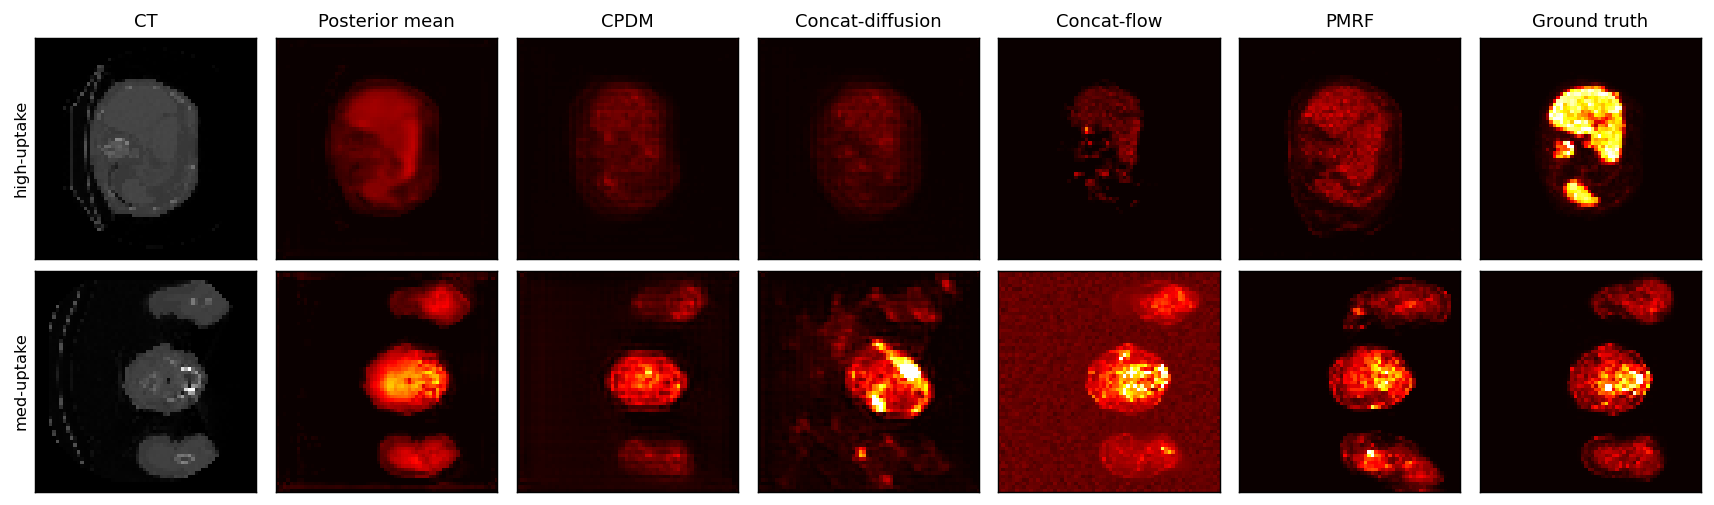
\includegraphics[width=\linewidth]{figures/qualitative_short.png}
\caption[Qualitative CT $\to$ PET, one high- and one medium-uptake slice]{Qualitative CT $\to$ PET
on matched test slices, one high-uptake (top) and one medium-uptake (bottom). Columns left to
right: CT input, posterior-mean anchor, CPDM (focal-attention fine-tune), concat-diffusion,
concat-flow, PMRF, ground truth. CT in grayscale, PET in a hot colormap (per-row shared $[0,1]$
stretch to the GT 99.5th percentile). The extended six-slice version is Figure~\ref{fig:app-qual}
in App.~\ref{app:qual}.}
\label{fig:qualitative}
\end{figure}

\begin{figure}[h]\centering
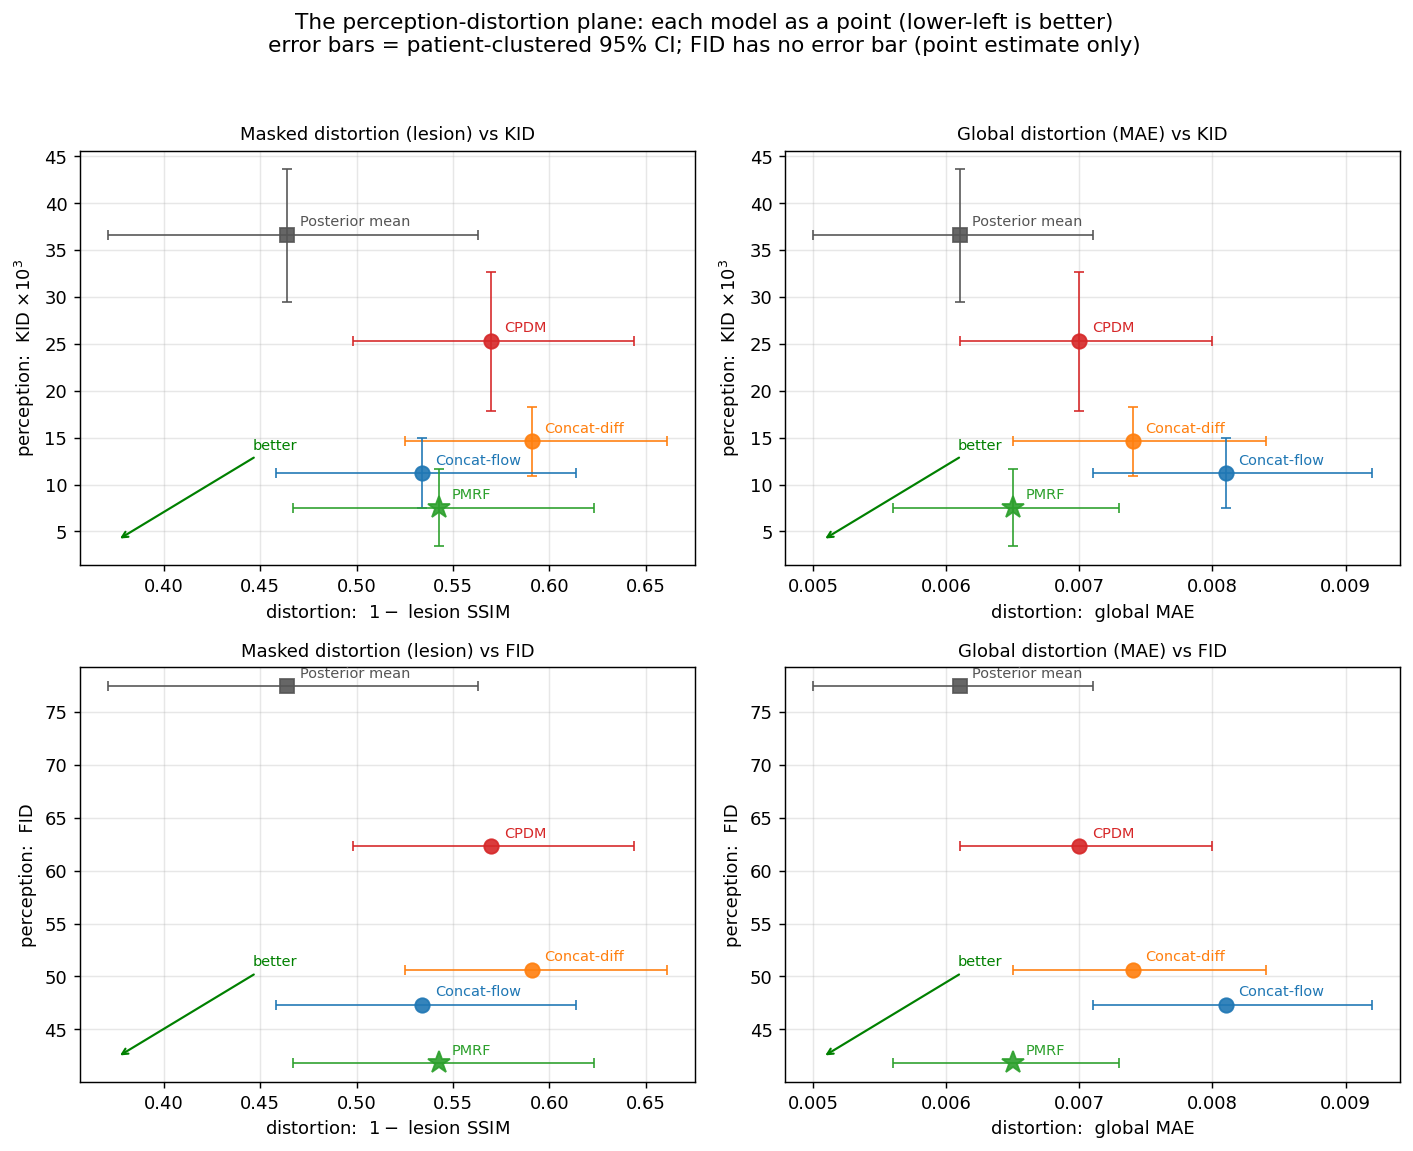
\includegraphics[width=\linewidth]{figures/pd_plane.png}
\caption[The perception--distortion plane, every model as a point]{The perception--distortion
plane with every model as a point; lower-left is best in all four panels. Columns vary the
distortion axis (masked $1-$lesion SSIM vs global MAE); rows vary the perception axis (KID vs
FID). Error bars are patient-clustered 95\% CIs; FID is a point estimate only
(Sec.~\ref{sec:stats}).}
\label{fig:pd-plane}
\end{figure}

\paragraph{The two-stage flow, visualised.} Figure~\ref{fig:pmrf-row} follows one high-uptake test
slice through PMRF's two stages. The Stage-1 posterior mean recovers where uptake belongs but
leaves it smooth and washed out, the blurry MSE-optimal estimate; the Stage-2 flow then adds the
missing high-frequency texture, moving the image onto the data manifold without displacing the
uptake, so the PMRF panel is visibly sharper than the posterior mean while staying close to the
ground truth. The full six-slice version is Figure~\ref{fig:app-pmrf} in App.~\ref{app:pmrf}.

\begin{figure}[H]\centering
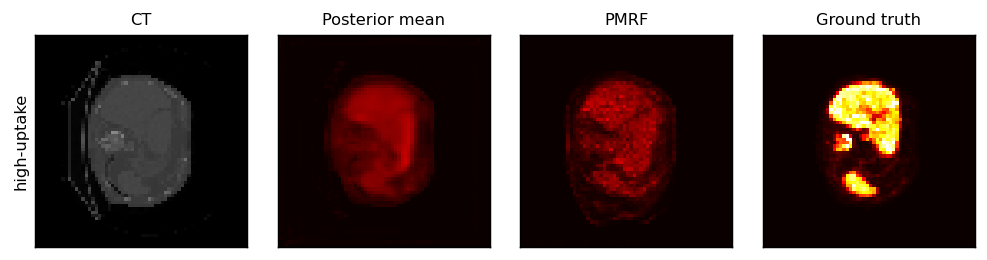
\includegraphics[width=\linewidth]{figures/appendix_pmrf_row.png}
\caption[One test slice through PMRF's two stages]{One test slice through PMRF's two stages:
CT, Stage-1 posterior mean, Stage-2 PMRF, ground truth.}
\label{fig:pmrf-row}
\end{figure}

\paragraph{When the domain prior helps, and when it does not.} Figure~\ref{fig:cpdm-row} follows
the same idea through CPDM's conditioning. The uninformative ``blob'' attention prior floods most
of the body, whereas the corrected focal prior localises to the true high-uptake region, and the
focal-conditioned output is correspondingly slightly better structured (H5). Even so, both CPDM
panels stay diffuse and low-contrast against the ground truth, the visual side of CPDM's weak
perception in Table~\ref{tab:results}. The full grid, including the attenuation map CPDM also
consumes, is Figure~\ref{fig:app-cpdm} in App.~\ref{app:cpdm}.

\begin{figure}[H]\centering
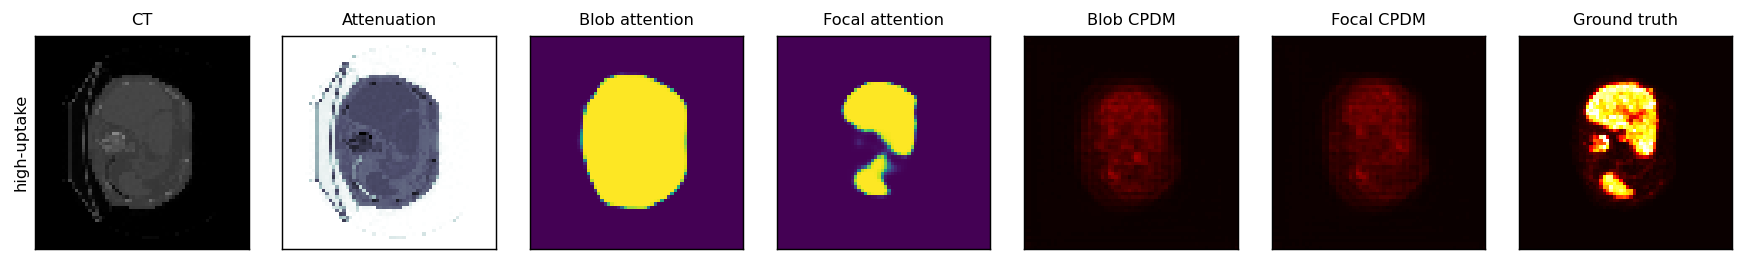
\includegraphics[width=\linewidth]{figures/appendix_cpdm_row.png}
\caption[One test slice through CPDM's conditioning]{One test slice through CPDM's conditioning:
CT, attenuation map, blob versus focal attention, blob versus focal CPDM output, ground truth.}
\label{fig:cpdm-row}
\end{figure}

\subsection{Training dynamics}
\label{sec:training-dynamics}
\paragraph{What ``validation loss'' denotes.} Each stage is monitored by the held-out counterpart
of its own training objective, so the term means a different quantity for each model. The
attention U-Net is validated with its Dice-plus-binary-cross-entropy loss; the VQGAN with its
reconstruction objective ($L_1$ plus the codebook commitment term, and, when enabled, the VGG-LPIPS
perceptual and adversarial terms); the posterior-mean U-Net, which also serves as PMRF's Stage~1,
with pixel MSE; CPDM and concatenation-conditioned diffusion with their latent denoising loss
(Brownian-bridge $L_1$ and $\varepsilon$-MSE respectively), computed on held-out latents; and the
two flows with held-out flow-matching loss. Because the objectives differ, validation-loss levels
are comparable only within a model, as a convergence signal, never across models.

Figure~\ref{fig:training-losses} shows the training and validation loss of all four
generators on a common layout. Read the shapes, not the absolute levels: the four
objectives differ (Brownian-bridge $L_1$, $\varepsilon$-MSE, and two flow-matching losses),
so the vertical scales are not comparable across panels. Every model's training loss
descends smoothly and its validation loss flattens, indicating convergence in each case. Two
patterns are worth noting. The two concatenation-conditioned models show a widening
train--validation gap late in training (validation loss drifting up while training loss keeps
falling), the mild over-fitting expected of a network with no strong inductive prior on this
modest dataset. PMRF, by contrast, keeps train and validation tightly coupled and at the
smallest absolute values, because its Stage-2 target $x_0-z_0$ is small by construction, the
flow only has to transport the posterior-mean estimate a short way onto the data manifold, not
because it is ``better trained'' than the others. The supporting stages shared across models (the
VQGAN autoencoder, the attention-UNet at best validation IoU \num{0.62} on the focal target, and
the posterior-mean U-Net that also serves as PMRF's Stage~1) all converge well before the
generators that consume them.

\paragraph{Latent loss is not image quality.} For the two latent-space diffusion models a subtlety
governs how the reported checkpoint is chosen. Their validation loss is measured in the VQGAN
latent, whereas the reported metrics live in pixel space, after the frozen decoder. The two need not
move together, and in the per-epoch validation metrics logged for CPDM in this work they did not:
the latent denoising loss kept falling after the decoded-image metrics (PSNR, SSIM) had peaked and
begun to drift down. This is expected rather than anomalous. A lower latent error is only a proxy for
image quality; the perception--distortion tradeoff establishes that pixel fidelity and perceptual
quality need not improve together~\parencite{blau2018perception,blaumichaeli2019rethinking}, and in a
latent model the frozen autoencoder sits between the latent and the image, so its
perceptually-trained decoder can trade pixel accuracy for
sharpness~\parencite{rombach2022ldm,esser2021vqgan}. Selecting the checkpoint by lowest latent
validation loss would therefore report a model past its image-quality peak, the pattern of a falling
validation loss alongside a falling PSNR that motivated this check. To avoid it, the two latent
models are checkpointed on the decoded validation metrics by which they are ultimately judged
(structural similarity and LPIPS), logged every epoch, rather than on the latent loss. This
separates ``training has converged'' (latent loss flat) from ``image quality is best''
(metric-selected checkpoint).

\begin{figure}[h]\centering
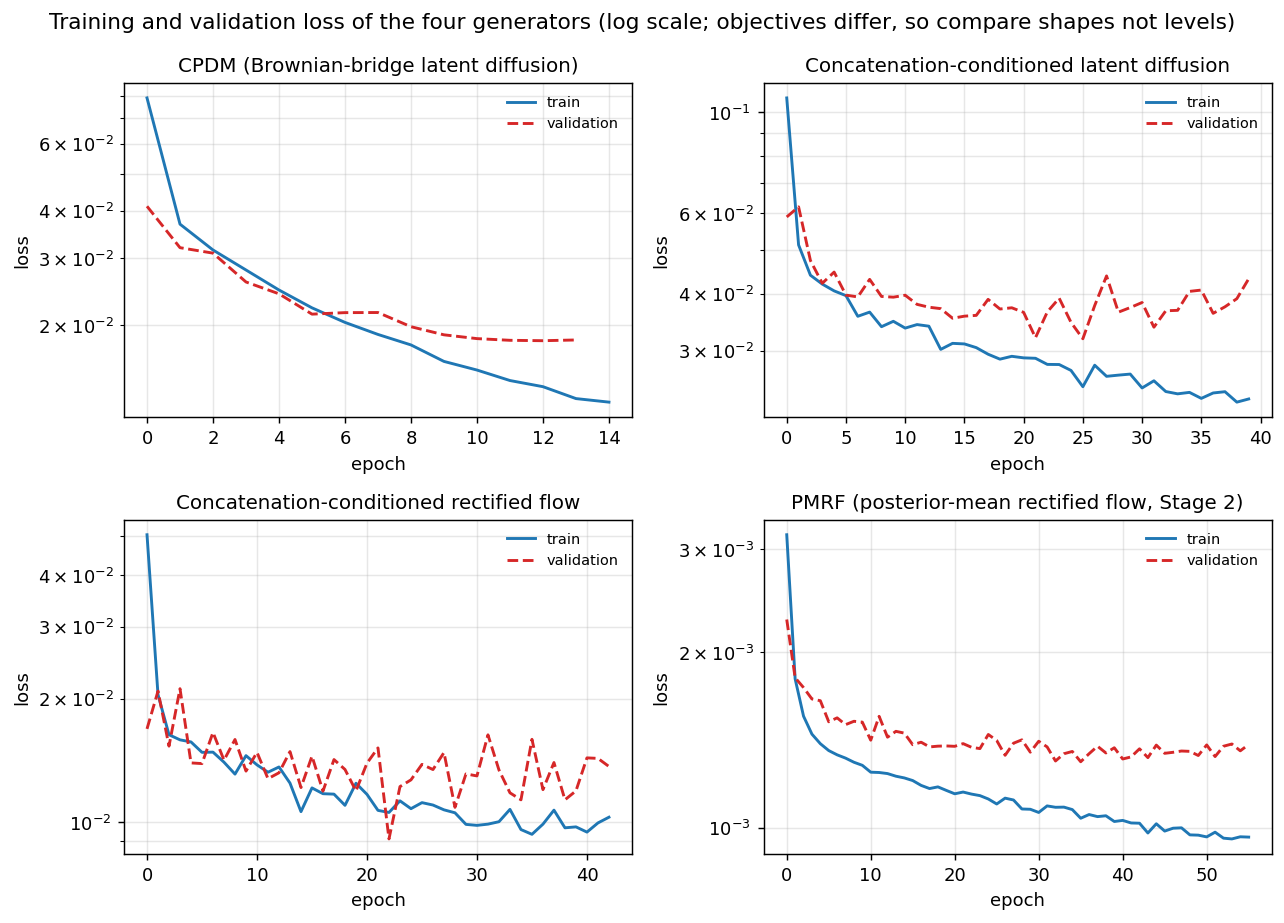
\includegraphics[width=\linewidth]{figures/training_losses.png}
\caption[Training and validation loss for the four generators]{Training (solid) and validation
(dashed) loss for each of the four generators, on a shared log-scale layout. Objectives differ
across models, so the panels are read by shape, not absolute level.}
\label{fig:training-losses}
\end{figure}

% ======================================================================
\section{Discussion}
\label{sec:discussion}

\paragraph{Where each model lands on the P--D plane.} Figure~\ref{fig:pd-plane} plots every model
as a point on this plane; the frontier it traces is the expected one.
The posterior-mean anchor sits at the distortion extreme: best MAE/SSIM on every tier but the
worst perception (FID \num{77.0}). PMRF occupies the most favourable knee of any
model, the lowest FID (\num{42.0}) and KID (\num{0.008}) overall, achieved while also holding
the best global SSIM (\num{0.890}) of any generator and near-best ROI distortion. This is
the posterior-mean-initialisation thesis of Sec.~\ref{sec:pmrf-theory} confirmed empirically:
starting the flow from an MSE-optimal estimate and learning only the short transport onto the
data manifold beats both the distortion anchor and the prior-free generators on perception. The
clearest controlled evidence is the flow-vs-flow pair, which share identical rectified-flow
machinery and differ only in their starting point: PMRF's posterior-mean init lifts
global SSIM from \num{0.816} (concat-flow, from noise) to \num{0.890} and FID from \num{46.9}
to \num{42.0}. Within the diffusion family CPDM and the concat model are close on distortion
(both share the VQGAN latent), but concat-diffusion is markedly better on perception.

\paragraph{Does the domain prior (CPDM) buy a better trade-off?} On this evidence, no.
CPDM's perception (FID \num{62.3}) is the worst of any generator and clearly behind the
prior-free concat-diffusion (FID \num{50.5}) that uses its exact latent with a $\sim$6$\times$
lighter denoiser ($\sim$16\,M vs.\ CPDM's $\sim$100\,M, both denoiser-only, the shared VQGAN is
frozen in both). The natural objection is that CPDM, by far the heaviest model (\num{100}\,M
trainable denoiser), was simply under-trained, but this was tested directly: a control CPDM trained from
scratch on the focal maps plateaued at the same level by epoch~15 (App.~\ref{app:cpdm-compare}),
so the deficit is not a convergence artefact but a genuine property of the model at this
budget. The priors therefore did not pay off here: the CT-derived attention and attenuation
maps do not give the Brownian bridge an advantage over plain concatenation. Whether they would
at GPU-scale resolution and capacity remains open, but on the present, converged evidence the
domain prior is not the deciding factor. One honest qualification: CPDM's weakness is specifically
one of distributional realism. On the per-image LPIPS, where a smooth output is penalised
less than in a distribution match, CPDM is level with the best generators (LPIPS \num{0.119},
statistically tied with concat-diffusion and PMRF), so the deficit is that CPDM's outputs do not
collectively look like real PET, not that any single output is perceptually far from its own
target.

\paragraph{How robust is CPDM's weak-perception position?} It is not an artefact of any single
training choice. The same diffuse, low-perception behaviour recurs across every variation of
the setup tested here: whether CPDM is fine-tuned or trained from scratch
(App.~\ref{app:cpdm-compare}), and under both the uninformative blob and the corrected focal
attention target (H5). That the deficit reproduces across conditioning quality and training
regime, and across independent runs, is what allows it to be attributed to the architecture and
the ill-posed CT-to-PET task at this budget rather than to under-training or one unlucky run. A controlled
study of why the domain-guided bridge lands where it does, for instance whether
warm-starting versus cold-starting biases a generator's position on the perception--distortion
plane, would need compute-matched arms and repeated seeds and is left to future work; the
single fine-tune-versus-scratch pair here is a convergence check, not such a test.

\paragraph{Does the masked metric change the ranking?} Yes, in the way the methodology
predicted. Global SSIM compresses the field into a narrow \num{0.82}--\num{0.91} band, but the
lesion tier, the $\sim$\num{2}\,\% of voxels that carry the diagnostic signal, spreads it
(\num{0.40}--\num{0.53}) and reorders the generators by point estimate: concat-flow's lesion
SSIM (\num{0.464}) is the highest of any generator there despite its worst global SSIM,
because its sharper (if noisier) output preserves focal structure the smoother models wash
out. This re-ordering is a point-estimate effect, the per-patient lesion CIs
(Table~\ref{tab:ci-compare}) overlap, so it is not established as a significant separation;
where masked metrics do significantly separate a pair is the paired CPDM$>$concat-diff
lesion contrast ($p_{\text{Holm}}\!=\!0.005$, Table~\ref{tab:hyptests}). Reporting only global
metrics would still have hidden the effect; the global-vs-lesion gap is the honest per-model
signal argued for in Sec.~\ref{sec:eval}.

\paragraph{Hypotheses revisited.} Table~\ref{tab:hypotheses} collects the verdicts, each backed
by the pre-specified contrast in Table~\ref{tab:hyptests}. The most informative is H2,
which is not supported: within the diffusion family the prior-free concat model is
significantly better on perception than the domain-guided Brownian bridge
($\Delta$KID $p_{\text{Holm}}\!=\!0.02$), and within the flow family PMRF's edge over concat-flow
is directional but does not survive the multiple-comparison correction
($p_{\text{Holm}}\!=\!0.14$), so the paradigm-native member out-performs plain concatenation
significantly in neither family. The diffusion result survives the obvious objection that CPDM, the heaviest
model, was under-trained: a from-scratch control plateaued at the same level
(App.~\ref{app:cpdm-compare}), and even the focal-corrected CPDM (FID \num{62.3}) does not reach
the prior-free concat-diffusion (\num{50.5}) that shares its latent. By contrast H3
holds with significance, PMRF beats both diffusion generators on KID
($p_{\text{Holm}}\!\le\!0.02$): on the present evidence a domain prior is neither necessary nor
sufficient for a better trade-off, whereas the posterior-mean initialisation of H3 clearly is.

\begin{table}[h]\centering\small
\caption{Hypotheses (Sec.~\ref{sec:hypotheses}) and their verdicts, with the deciding statistical
contrast (Table~\ref{tab:hyptests}); $^*$ marks Holm-corrected $p<0.05$.}
\label{tab:hypotheses}
\begin{tabular}{p{0.08\linewidth} p{0.42\linewidth} p{0.28\linewidth} p{0.12\linewidth}}
\toprule
Hyp. & Prediction & Deciding evidence & Verdict \\
\midrule
H2 & Paradigm-native $>$ concatenation within family & diffusion: concat-diff beats CPDM on KID ($p_{\text{Holm}}\!=\!0.02$); flow: PMRF $>$ concat-flow directionally but n.s.\ ($p_{\text{Holm}}\!=\!0.14$) & not supported (diffusion refuted$^*$; flow n.s.) \\
H3 & PM-initialised flow reaches the best knee & PMRF lowest FID/KID (\num{42.0}/\num{0.008}); KID beats both diffusion generators$^*$; best generator global SSIM & confirmed \\
H4 & Masked metrics re-rank vs.\ global & lesion tier re-orders the point estimates (concat-flow highest despite worst global SSIM) and the paired CPDM$>$concat-diff lesion contrast is significant, though the marginal lesion CIs overlap & confirmed (re-ordering) \\
H5 & Domain prior helps only if informative & focal $>$ blob on active SSIM$^*$ ($p_{\text{Holm}}\!=\!0.005$); KID gain n.s. & confirmed (distortion) \\
\bottomrule
\end{tabular}
\end{table}

\paragraph{Limitations.}
\label{sec:limitations}
A few caveats bound these conclusions. The models are trained and evaluated on single 2D slices,
so no through-plane context is used, whereas whole-body PET has 3D structure a slice model cannot
exploit. The masked metrics rely on fixed SUV thresholds ($>0.5$ for active tissue, $>2.5$ for
lesion); these are reasonable but not swept, and a sensitivity analysis would strengthen the
tier-wise claims. The shared evaluation uses \num{300} slices from \num{12} held-out patients
(\num{7} FDG, \num{5} PSMA); every model is scored on the identical slices with patient-clustered
uncertainty (Sec.~\ref{sec:stats}), which is enough to separate the models statistically but
modest for reading the absolute numbers as whole-population estimates, so a larger
multi-institutional test set would tighten the intervals further. The across-family
diffusion-versus-flow comparison is confounded by the latent-versus-pixel design choice: the two
diffusion models operate in the VQGAN latent, the two flows in pixel space. Isolating that
latent-versus-pixel axis is deliberately not the aim of this study, which controls the conditioning
mechanism within each family (both members of a family share the same representation) and therefore
treats only the within-family contrasts as clean tests, keeping the cross-family comparison
descriptive. The distinction is not cosmetic: a latent generator can never render a PET more
faithfully than its frozen autoencoder can reconstruct a real one, a reconstruction ceiling inherent
to latent generative models~\parencite{rombach2022ldm,esser2021vqgan} that the pixel-space models do
not face. Part of why the two latent diffusion models trail on perception may
therefore be this autoencoder bottleneck rather than the diffusion paradigm itself, which would
place some of the observed spread on the representation axis this thesis does not disentangle.
Separating the two, with a pixel-space diffusion arm or a higher-fidelity autoencoder, is left to
future work. Finally, at $64\times64$ the
synthetic PET is not sharp enough to satisfy a radiologist; this study compares architectures on a
common controlled footing rather than against paper-state-of-the-art absolute quality.

% ======================================================================
\section{Conclusion}
\label{sec:conclusion}
This work compared four generative architectures, two diffusion (Brownian-bridge CPDM,
concatenation-conditioned latent DDPM) and two flow (concatenation-conditioned rectified flow,
posterior-mean rectified flow), for CT-to-PET synthesis, with a deterministic posterior-mean
U-Net as a distortion anchor, all trained CPU-only and judged by one shared global-plus-masked
ruler. The models spread out along the perception--distortion plane as theory predicts: the
posterior-mean anchor is distortion-optimal but perceptually poor, and \textbf{PMRF reaches the
most favourable knee}, the best perceptual realism of any model (FID \num{42.0}, KID
\num{0.008}) while also holding the best global structural similarity of any generator,
confirming that initialising a flow from an MSE-optimal estimate beats both the anchor and the
prior-free generators on the same machinery. Domain guidance (CPDM) did not buy a better
trade-off at the budget tested, and, since a from-scratch control plateaued at the same level,
this reflects the model at convergence rather than an under-trained checkpoint; whether the
priors would help at GPU-scale resolution and capacity remains open.
Methodologically, the central practical takeaway is that the global-vs-masked gap is
essential: on a target that is \num{89}\,\% near-zero, global metrics compress and even
reorder the models relative to the lesion-region metrics that reflect diagnostic value: honest reporting on sparse functional images requires measuring where the signal actually is.

% ======================================================================
\clearpage
\printbibliography

% ======================================================================
\clearpage
\section*{Declaration of AI Usage}
\addcontentsline{toc}{section}{Declaration of AI Usage}
Artificial-intelligence tools were used in the preparation of this thesis in three ways: to help
put the author's own ideas and results into written form, to support the author's understanding
and consolidation of background material, and to assist with formatting and \LaTeX{}. The research
questions, the experimental design, the implementation, the analysis, and the conclusions are the
author's own, and all outputs produced with such assistance were reviewed and verified by the
author.

% ======================================================================
\clearpage
\appendix
\section{Appendix}
\label{app:appendix}

\subsection{Extended qualitative comparison (all models)}
\label{app:qual}
\begin{figure}[!ht]\centering
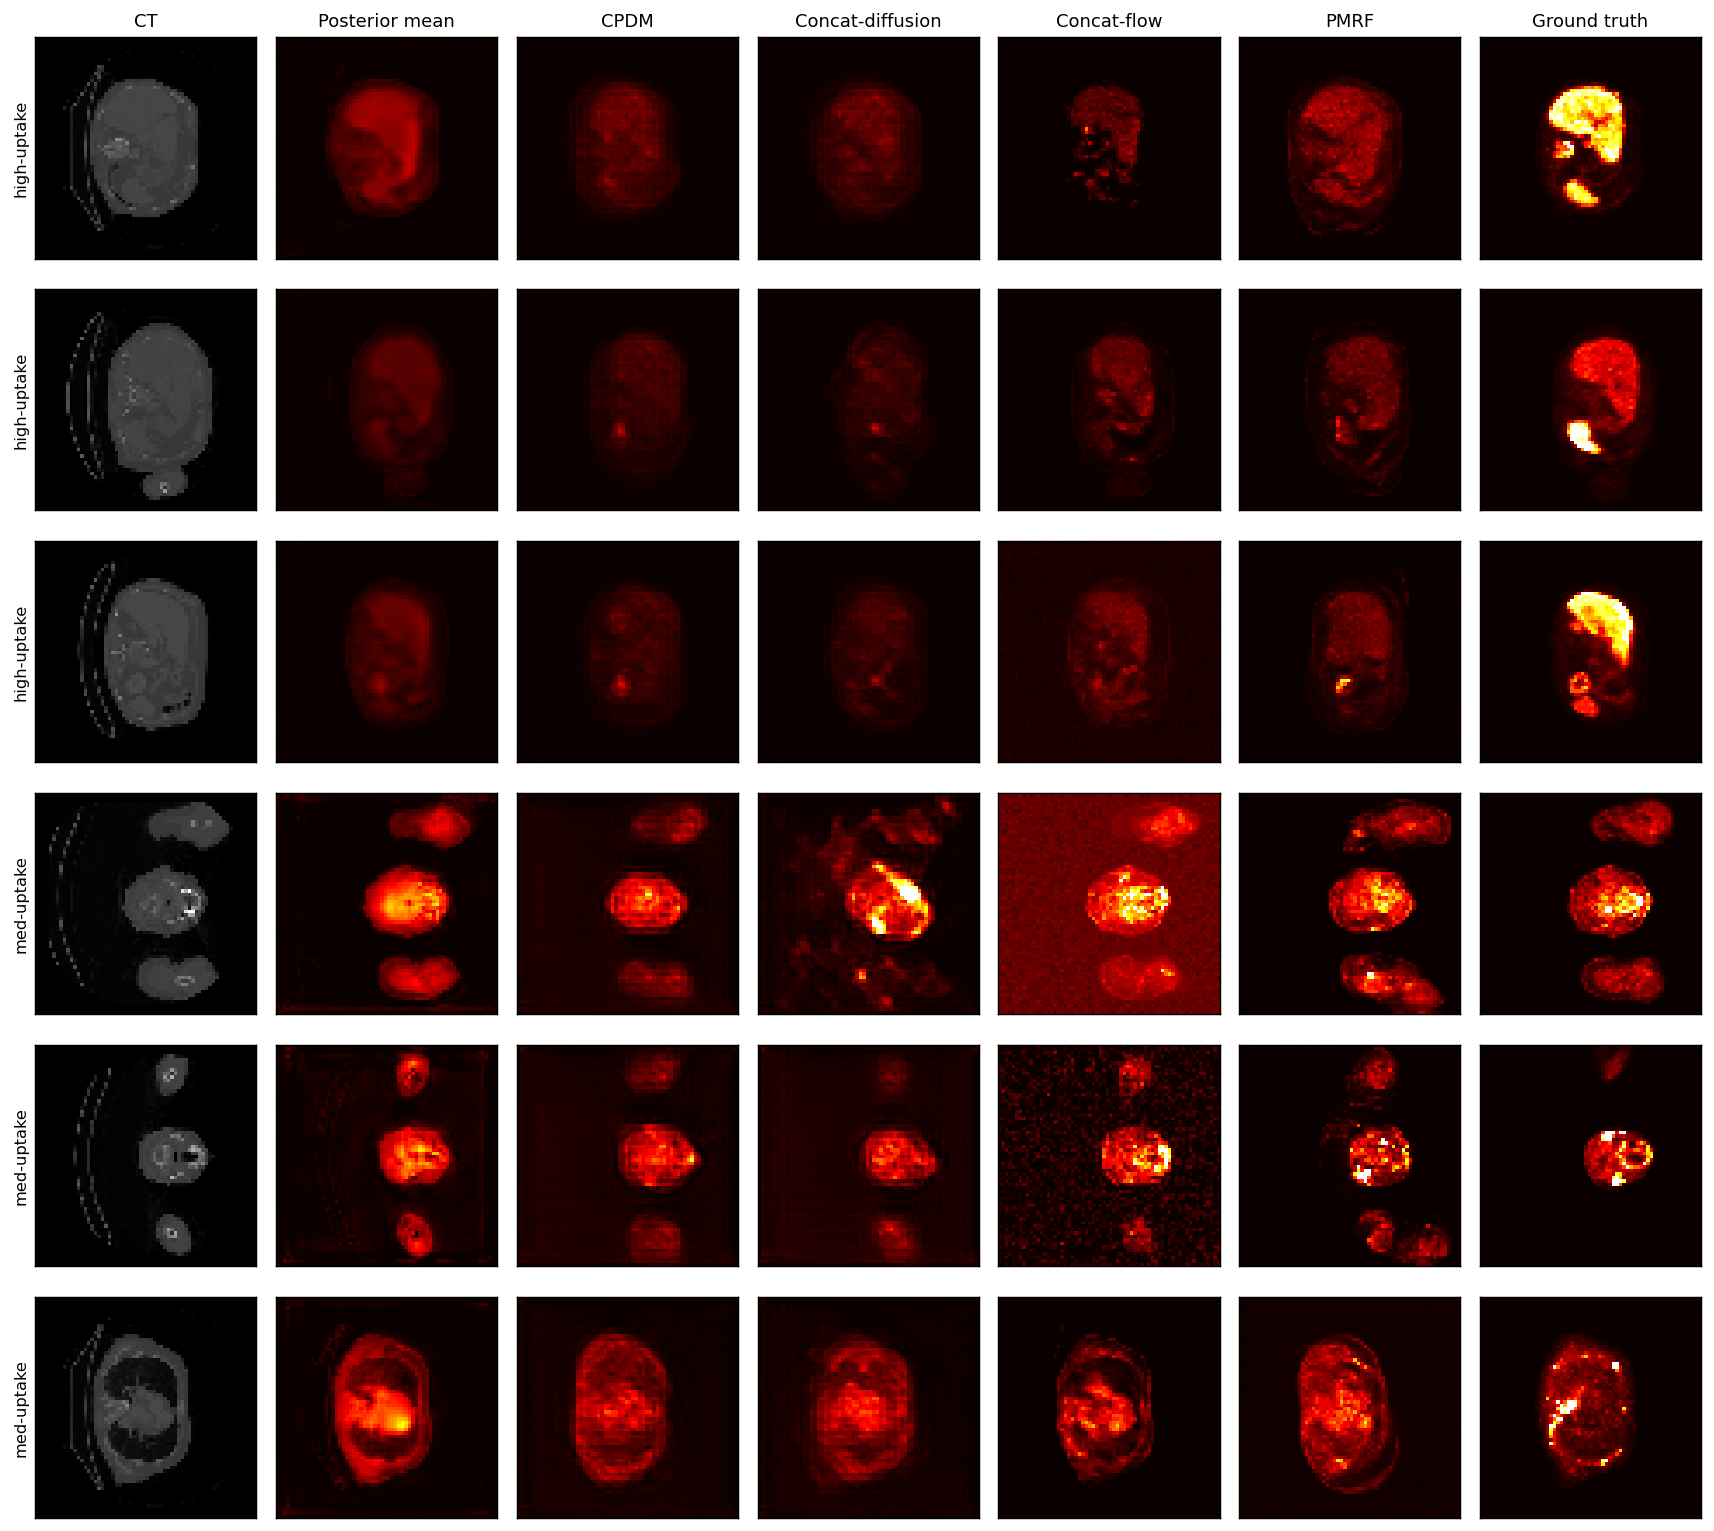
\includegraphics[width=\linewidth,height=0.72\textheight,keepaspectratio]{figures/qualitative.png}
\caption[Extended qualitative comparison across all models]{Extended qualitative comparison:
three high-uptake (top) and three medium-uptake (bottom) test slices. Columns: CT input,
posterior-mean anchor, CPDM (focal), concat-diffusion, concat-flow, PMRF, ground truth (same
hot colormap and per-row $[0,1]$ stretch as Figure~\ref{fig:qualitative}).}
\label{fig:app-qual}
\end{figure}

\clearpage
\subsection{Qualitative PMRF two-stage panels}
\label{app:pmrf}
\begin{figure}[!ht]\centering
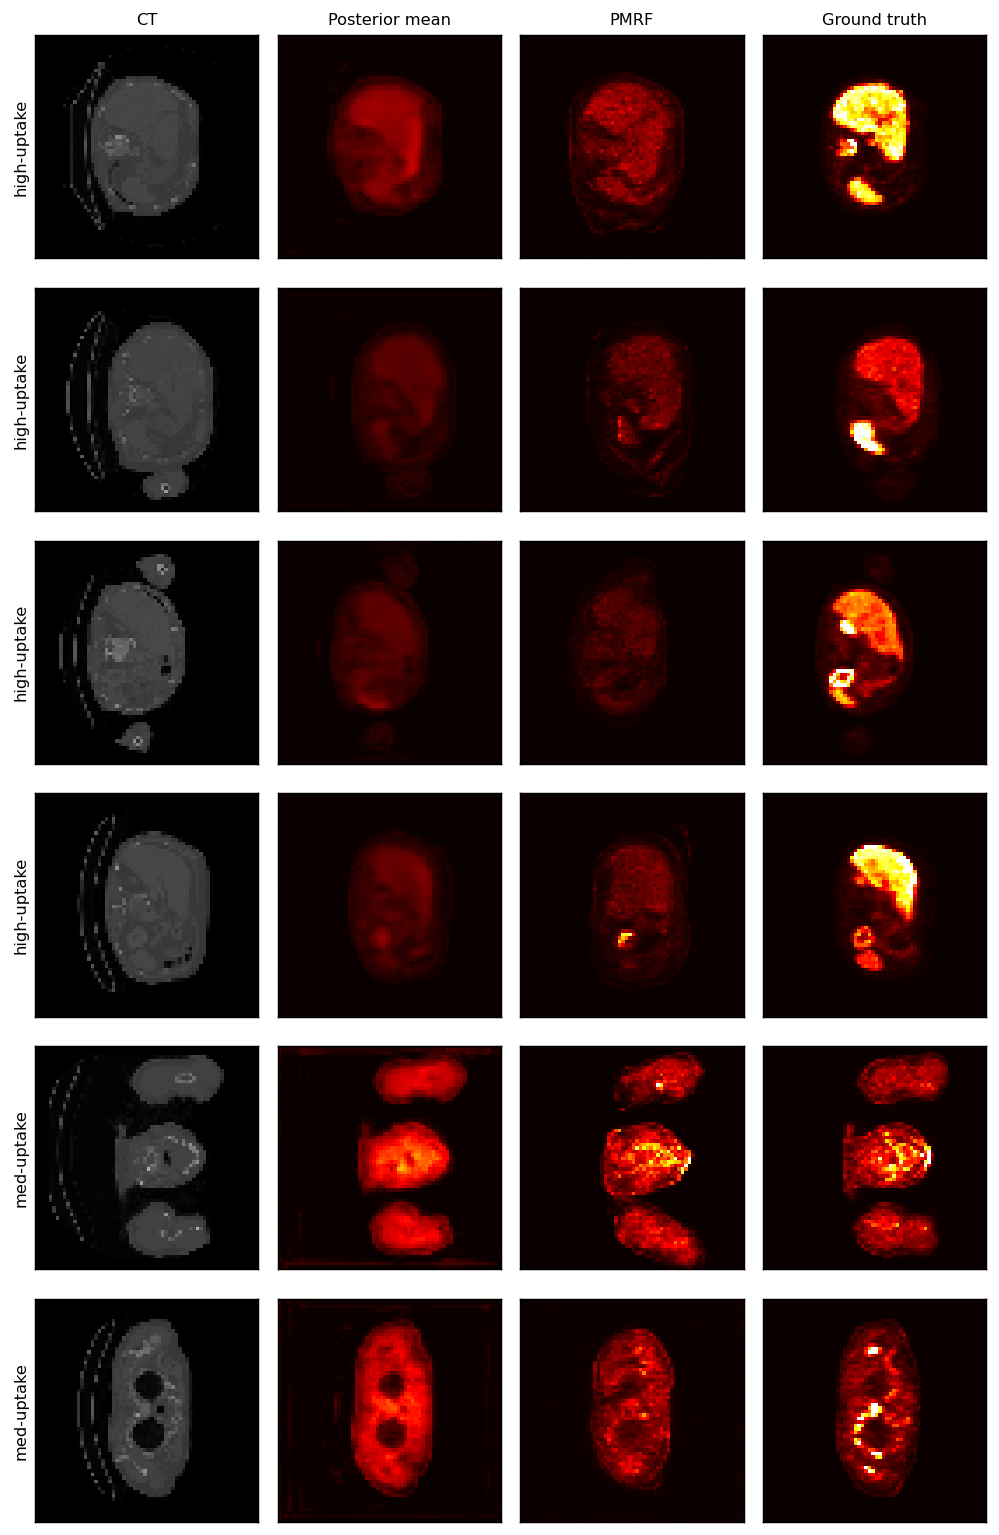
\includegraphics[width=\linewidth,height=0.72\textheight,keepaspectratio]{figures/appendix_pmrf.png}
\caption[PMRF two-stage panels]{PMRF two-stage panels. Columns: CT input, the Stage-1 posterior-mean U-Net
(MSE-optimal, deliberately smooth), the Stage-2 PMRF refiner, and the ground truth. Rows: high-
and medium-uptake test slices; PET in a hot colormap (per-row $[0,1]$ stretch to the GT 99.5th
percentile).}
\label{fig:app-pmrf}
\end{figure}

\clearpage
\subsection{CPDM conditioning and the attention-map correction}
\label{app:cpdm}
\begin{figure}[!ht]\centering
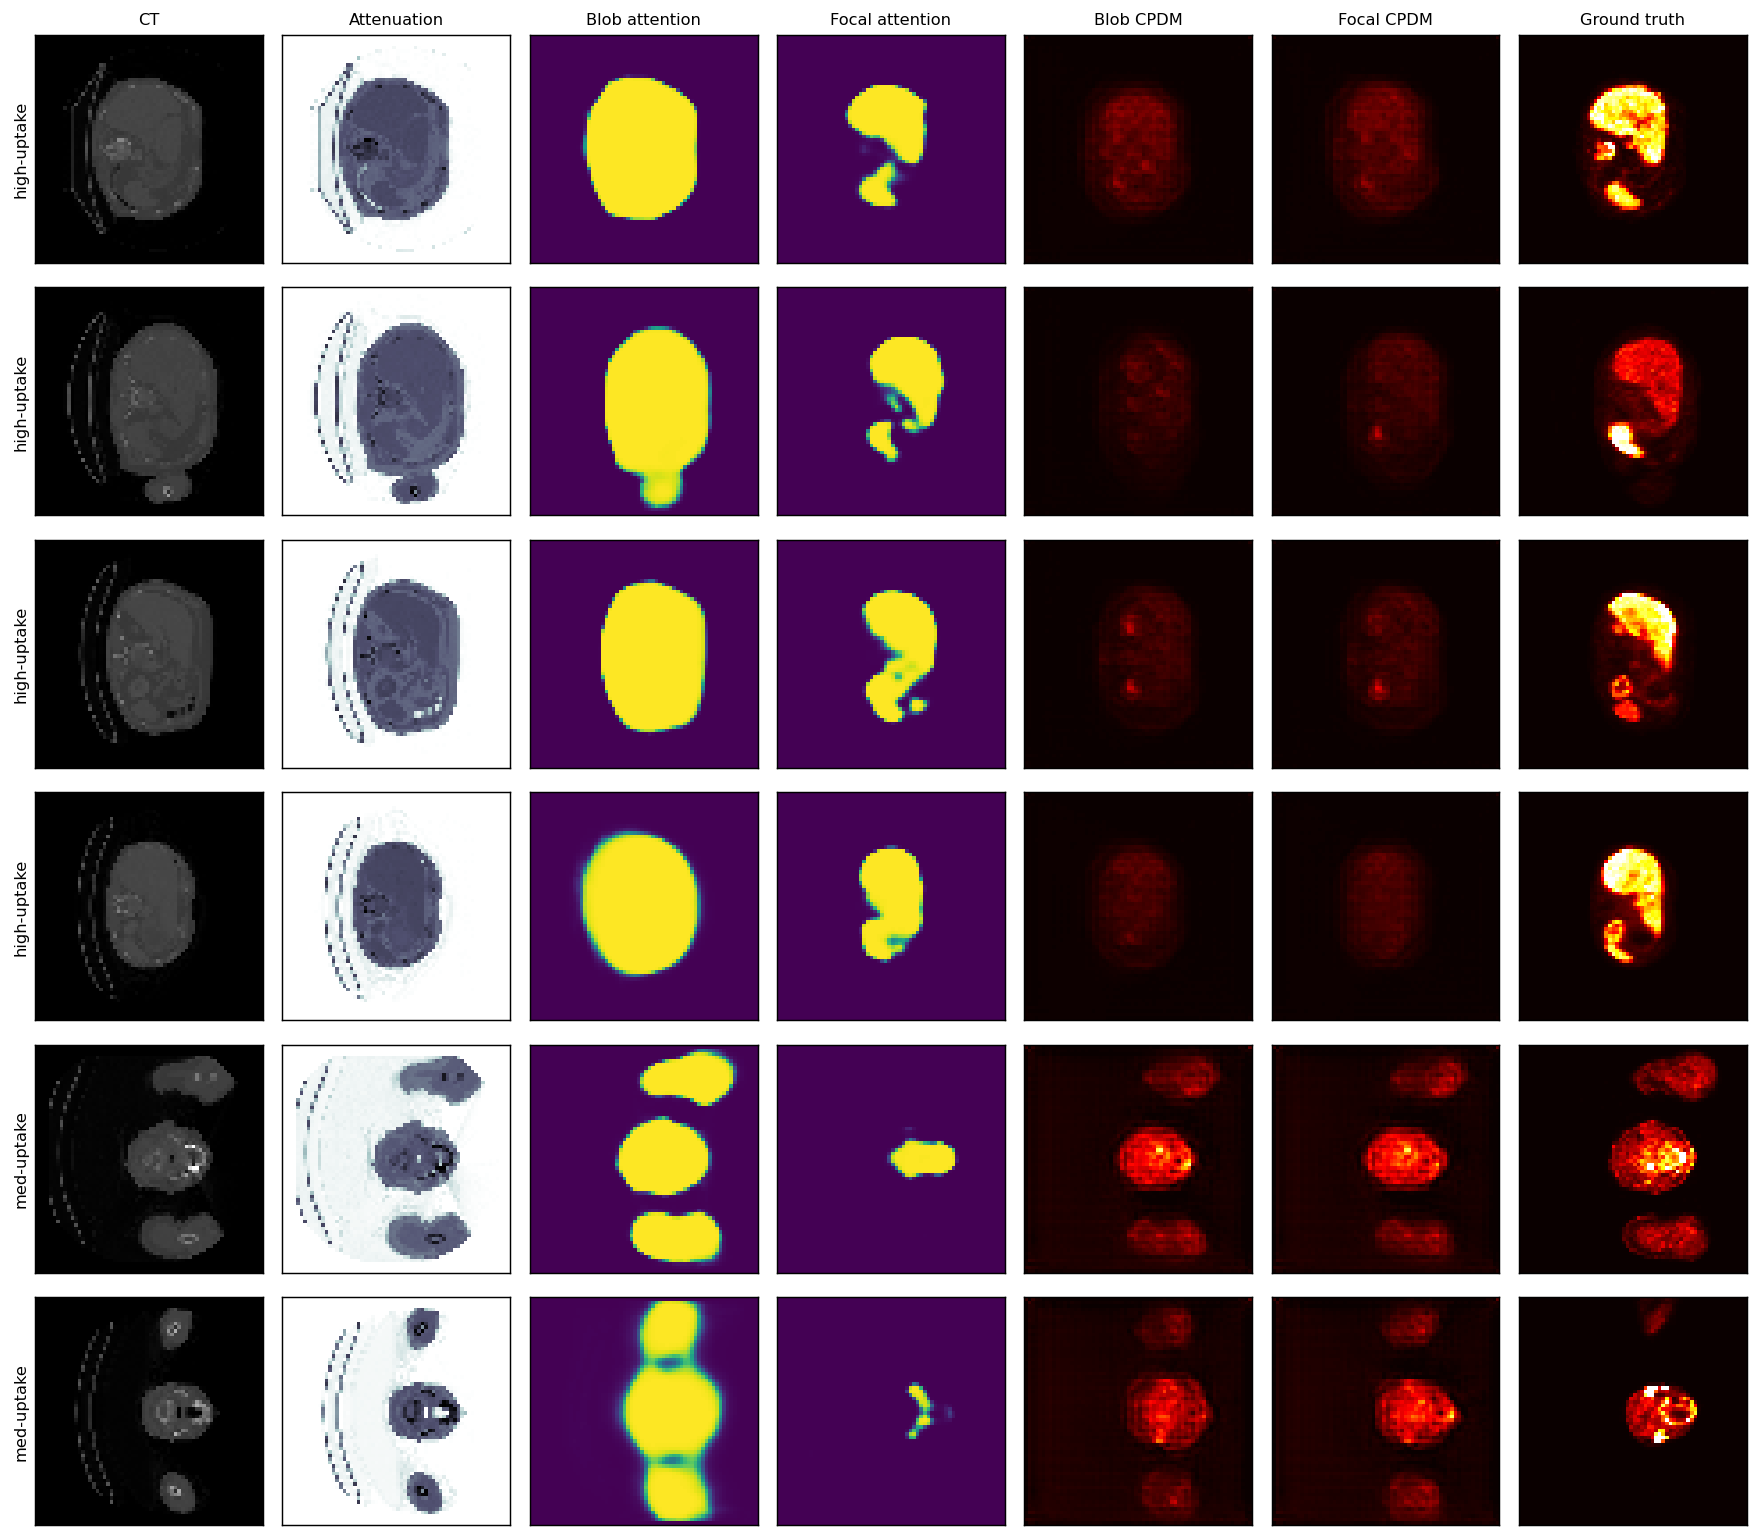
\includegraphics[width=\linewidth,height=0.72\textheight,keepaspectratio]{figures/appendix_cpdm.png}
\caption[CPDM conditioning and the blob-vs-focal attention fix]{CPDM conditioning and the
blob-vs-focal attention fix (Sec.~\ref{sec:cpdm-method}). Columns: CT input; the CT-derived
511\,keV attenuation map (shared by both runs); the original blob attention map (PET$>$75th
percentile over the whole frame, effectively the body outline); the corrected focal attention map
(SUV$>$\num{2.0}, localised on high-uptake organs); the resulting blob and focal CPDM outputs; and
the ground truth.}
\label{fig:app-cpdm}
\end{figure}

\clearpage
\subsection{CPDM convergence control: fine-tuned vs from-scratch focal training}
\label{app:cpdm-compare}
To rule out that CPDM's weak perception is an under-training artefact, a control CPDM was
trained from scratch on the focal attention maps (rather than fine-tuned from the blob
checkpoint). Its per-epoch validation LPIPS fell from \num{0.28} to \num{0.12} and plateaued by
epoch~15, and on the shared manifest it matches the fine-tuned model on the distortion tiers
(global SSIM \num{0.880} vs \num{0.876}) while being slightly worse on perception (FID
\num{68.2} vs \num{62.3}, KID \num{0.030} vs \num{0.025}). Both convergence paths therefore land
at the same weak-perception regime, so the reported (fine-tuned) CPDM is representative of the
architecture at this budget, not an under-trained checkpoint. Fig.~\ref{fig:app-cpdm-compare}
shows the two are visually near-identical: both collapse the bright focal uptake into a dim,
diffuse cloud.

\begin{figure}[!ht]\centering
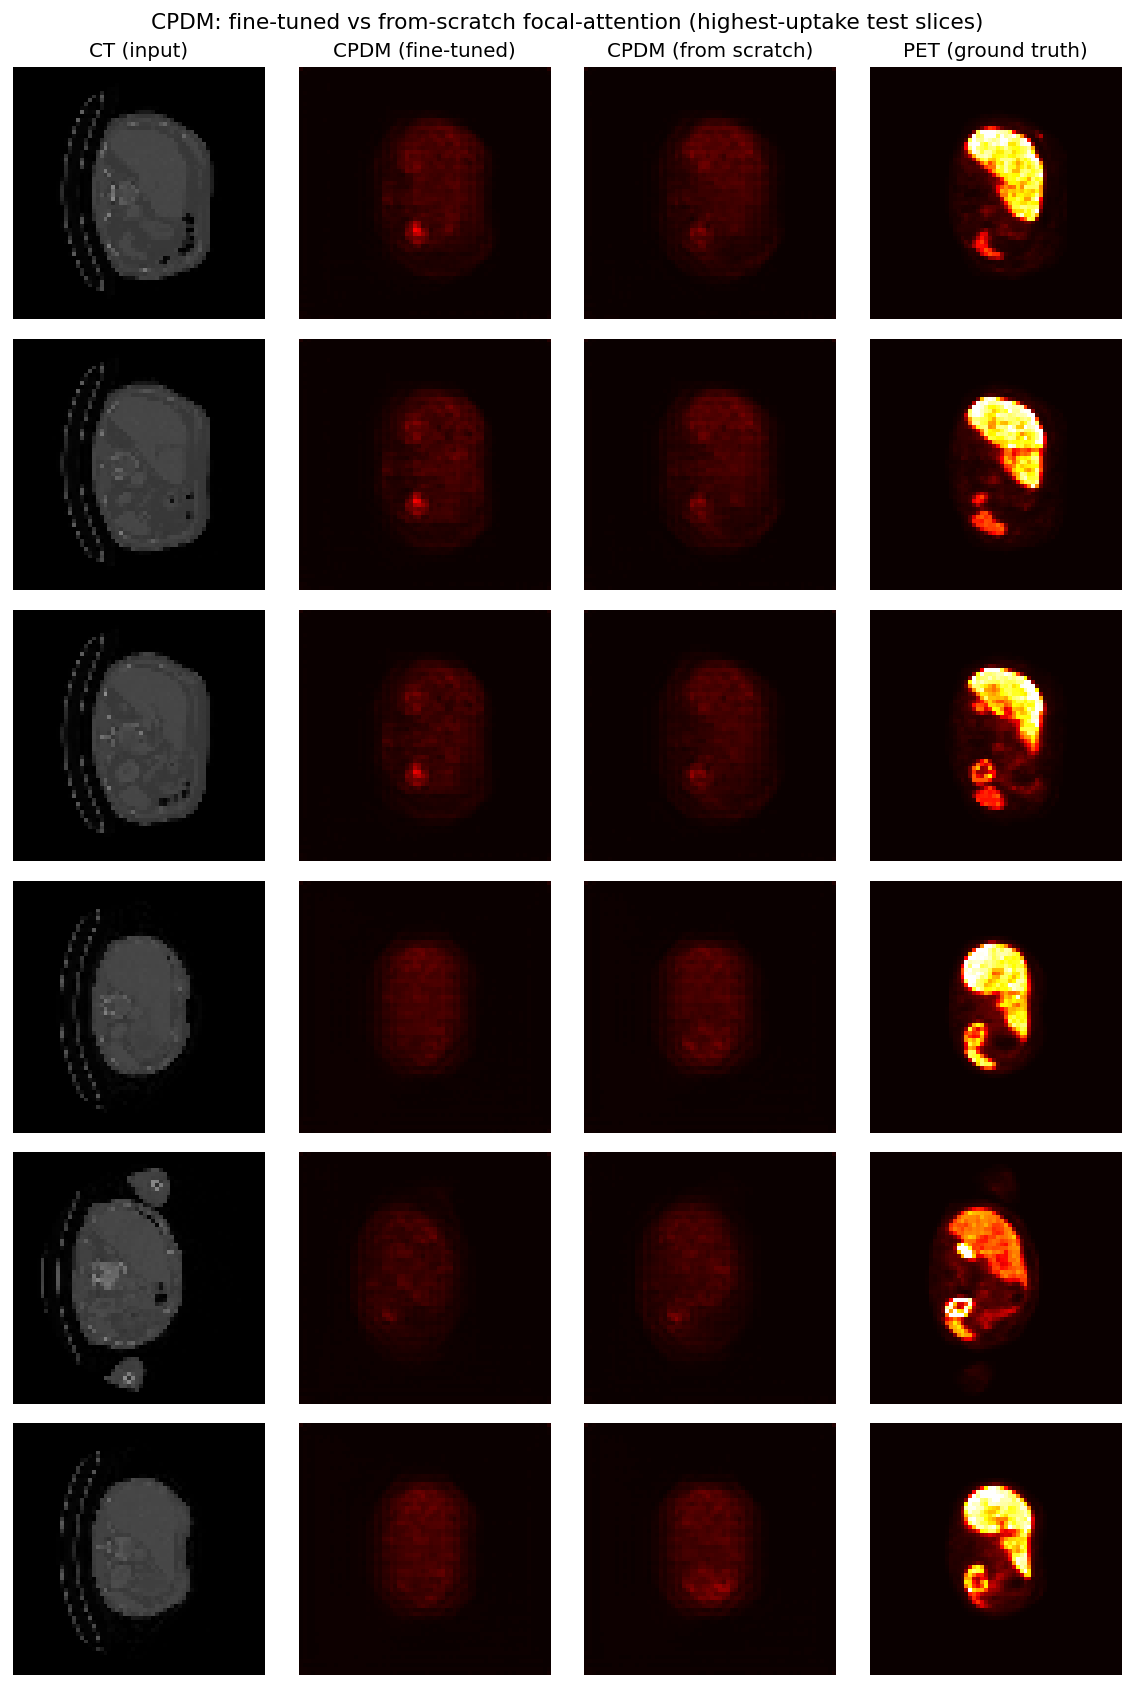
\includegraphics[width=\linewidth,height=0.58\textheight,keepaspectratio]{figures/cpdm_scratch_vs_finetune.png}
\caption[CPDM fine-tuned versus trained from scratch]{CPDM fine-tuned (from the blob checkpoint)
versus trained from scratch, both on the corrected focal attention maps, on the highest-uptake
test slices. Columns: CT input; fine-tuned CPDM; from-scratch CPDM; ground-truth PET (hot
colormap, per-row stretch to the GT $99.5$th percentile).}
\label{fig:app-cpdm-compare}
\end{figure}

\clearpage
\subsection{Hyperparameters}
\label{app:hyperparams}
The settings below were largely inherited from the source papers (CPDM~\parencite{nguyen2025cpdm},
PMRF~\parencite{ohayon2025pmrf}) and adapted for single-CPU training rather than tuned by search,
which the compute budget did not allow. Batch sizes and epoch caps reflect that budget; gradient
clipping at \num{1.0} and $64\times64$ inputs in $[-1,1]$ are common to all runs, and every model
draws from the identical shared head--torso set (Sec.~\ref{sec:dataset}) with the same train/val
caps, so no model is given a data advantage. Two shared stages (the frozen VQGAN and the CPDM-only
attention U-Net) are listed separately in Table~\ref{tab:hp-support}; the generators and the
posterior-mean anchor are in Table~\ref{tab:hp-gen}.

\begin{table}[h]\centering\footnotesize
\setlength{\tabcolsep}{3.5pt}
\renewcommand{\arraystretch}{1.25}
\caption[Generator and anchor hyperparameters]{Training hyperparameters of the four generators and
the posterior-mean distortion anchor. Parameter counts are trainable denoiser/network parameters
(the shared VQGAN is frozen in the two latent models). ES = early-stopping patience (epochs).}
\label{tab:hp-gen}
\begin{tabular}{p{0.115\linewidth} p{0.05\linewidth} p{0.235\linewidth} p{0.20\linewidth} p{0.10\linewidth} p{0.035\linewidth} p{0.125\linewidth}}
\toprule
Model & Space & Backbone (params) & Objective / sampling & Optim., lr & Batch & Schedule, ES \\
\midrule
CPDM (Diff.~1) & latent & U-Net $m{=}128$, mult $(1,2,3,4)$, attn.\ @$\{8,4\}$, in${=}12$ ($\sim$100\,M) & Brownian-bridge $L_1$, gradient obj.; 1000 train / 200 sampling & Adam $10^{-4}$, wd 0 & 8 & plateau ($\times0.5$, pat.\ 3000); EMA 0.995 @5k; ES 25 \\
Concat-diff. (Diff.~2) & latent & U-Net $m{=}64$, mult $(1,2,4)$, no attn., in${=}8$ ($\sim$16\,M) & $\varepsilon$-DDPM, linear $\beta$ $10^{-4}{\to}2{\times}10^{-2}$; 1000 train / 200 DDIM & AdamW $5{\times}10^{-4}$ & 8 & 100 epochs \\
Concat-flow (Flow~1) & pixel & ResUNet base 32, mult $(1,2,4,8)$, in${=}2$ ($\sim$13.5\,M) & flow matching; $z_0$ noise; $K{=}200$ Euler & AdamW $5{\times}10^{-4}$ & 64 & cosine; ES 20 \\
PMRF (Flow~2) & pixel & ResUNet base 32, mult $(1,2,4,8)$ refiner ($\sim$13.5\,M) + Stage-1 PM & flow matching; $z_0{=}\text{PM}{+}\sigma_s\varepsilon$, $\sigma_s{=}0.1$; $K{=}200$ & AdamW $5{\times}10^{-4}$ & 64 & cosine; ES 20 \\
PM U-Net (anchor / PMRF Stage 1) & pixel & ResUNet base 32, mult $(1,2,4,8)$ ($\sim$3.4\,M) & pixel MSE & AdamW $5{\times}10^{-4}$ & 128 & cosine; ES 20 \\
\bottomrule
\end{tabular}
\end{table}

\begin{table}[h]\centering\footnotesize
\setlength{\tabcolsep}{4pt}
\renewcommand{\arraystretch}{1.25}
\caption[Shared supporting-stage hyperparameters]{The two shared stages consumed by the latent
models. The VQGAN is frozen into CPDM and concat-diffusion; the attention U-Net supplies CPDM's
focal prior only.}
\label{tab:hp-support}
\begin{tabular}{p{0.13\linewidth} p{0.25\linewidth} p{0.19\linewidth} p{0.12\linewidth} p{0.045\linewidth} p{0.15\linewidth}}
\toprule
Stage & Backbone & Loss & Optim., lr & Batch & Notes \\
\midrule
VQGAN (frozen) & enc/dec ch 128, mult $(1,2,4)$ $\to$ latent $4{\times}16{\times}16$, 2 res-blocks, codebook $8192{\times}4$ & $L_1$ + codebook ($\beta{=}0.25$) + VGG-LPIPS (0.1) & Adam $10^{-4}$, $\beta(0.5,0.9)$ & 16 & $\le$100 epochs; sharper decode \\
Attention U-Net (CPDM) & smp U-Net, ResNet34 enc.\ + scSE dec., dropout 0.1 & 0.7 Dice + 0.3 BCE & $10^{-3}$, cosine & 32 & target focal SUV$>$2.0; $\le$50 epochs \\
\bottomrule
\end{tabular}
\end{table}

\end{document}
